\clearpage
\section{Appendix}
\renewcommand{\thefigure}{A.\arabic{figure}}
\renewcommand{\thetable}{A.\arabic{table}}
\subsection{Experimental Setup} \label{app:setup}
\textbf{Task setup.}
We evaluate AgentSquare and compared methods on six representative tasks covering four key domains which are widely adopted by existing LLM agent benchmarks~\citep{ma2024agentboard,xi2024agentgym}: 
\begin{itemize}[leftmargin=*]
    \item \textbf{Embodied:} ALFWorld~\citep{shridhar2021alfworld} with text-based household tasks where agents navigate and interact with objects using text commands, ScienceWorld~\citep{wang2022scienceworld} with interactive science tasks requiring agents to navigate rooms and perform experiments, testing scientific commonsense; 
    \item \textbf{Game:} PDDL~\citep{ma2024agentboard} including many strategic games where agents use PDDL expressions to complete tasks; 
    \item \textbf{Web:} WebShop~\citep{yao2022webshop} focusing on online shopping tasks where agents browse and purchase products based on user instructions; 
    \item \textbf{Tool:} TravelPlanner~\citep{xie2024travelplanner} with many travel planning tasks where agents use tools and data to create detailed plans, (6)M3ToolEval~\citep{wang2024executable} including complex tasks requiring multi-turn interactions with multiple tools.
\end{itemize}
The specific performance evaluation metric varies in different tasks, following the evaluation settings in their original work. Specifically, the evaluation metric is ``success rate'' for ALFWorld and M3ToolEval, ``task score (defined as the average reward obtained across episodes)'' for Webshop, ``progress rate'' for SciWorld and PDDL, and ``micro pass rate'' for TravelPlanner.

\textbf{Baselines.}
We compare AgentSquare with four types of baselines:
\begin{itemize}[leftmargin=*]
    \item \textbf{Hand-crafted agents.} We compare with 12 hand-crafted agents including CoT~\citep{wei2022chain}, CoT-SC~\citep{wang2023selfconsistency}, Self-refine~\citep{madaan2024self}, ToT~\citep{yao2024tree}, Step back~\citep{zheng2024take}, Thought propagation~\citep{yu2024thought}, HuggingGPT~\citep{shen2024hugginggpt}, Voyager~\citep{wang2024voyager}, Generative Agents~\citep{park2023generative}, DEPS~\citep{wang2024describe}, OPENAGI~\citep{ge2024openagi}and Dilu~\citep{wen2024dilu}. 
    \item \textbf{Module search methods.} We compare with two module-level agent optimization methods including the random combination of existing modules and Bayesian~\citep{zhou2019bayesnas} module combination optimization inspired by Bayesian optimization in NAS~\citep{white2021bananas}.
    \item \textbf{Prompt search methods.} 
    We select OPRO~\citep{yang2024large} as a representative prompt-level optimization approach, which leverages LLMs as optimizers by generating and refining instructions through iterative prompts.
    \item \textbf{Agent search methods.} We select ADAS~\citep{hu2024automated} which optimizes the entire agentic system in code space as the agent search baseline. We use the official code of ADAS and make slight modifications to adapt it to our tasks. 
    % The modifications are mainly on three aspects: (1) adjusting the task descriptions, instructions and examples in the meta prompt; (2) replacing the fitness value of each agent with its performance on our tasks; and (3) changing the evaluation procedure to align with our tasks.
\end{itemize}

\textbf{AgentSquare setup.}
We implement AgentSquare and conduct experiments using both GPT-3.5-turbo-0125 and GPT-4o~\citep{achiam2023gpt}. To ensure a fair comparison, we use the same number of few-shot examples across all methods. The initial agent is set as a random module combination, and the search process terminates after 5 consecutive iterations without performance improvement.

\begin{algorithm}[t!] 
% \SetAlgoNoLine 
\caption{Algorithm of AgentSquare} 
\label{alg}
% \LinesNumbered 
\KwIn{
Initial agent $A_0$, targeted task descriptions $d$, maximum evolution episode $K$,  population size $N$ per evolution phase, standardized module pools $\{\mathbb{P}, \mathbb{R}, \mathbb{T}, \mathbb{M}\}$, experience pool $\mathbb{E}$ 
}
\KwOut{The evolved agent $A^*$}
$t \leftarrow 1$ \tcp{Current search episode}
$A_e^0 \leftarrow A_0$  \tcp{Initialization of the module evolution phase} 
\While{$t \leq K$}{
$\{A_e^1,A_e^2,...,A_e^N\} \leftarrow \pi_{\xi} (A_e^0, d, N, \mathbb{P}, \mathbb{R}, \mathbb{T}, \mathbb{M}, \mathbb{E})$ 
\tcp{Module evolution}
$A_r^0 \leftarrow \argmax\{{Eval}_d(A_e^0), {Eval}_d(A_e^1),...,{Eval}_d(A_e^N)\}$  \tcp{Select the best-performing generated agent} 
$\{A_r^1,A_r^2,...,A_r^N\} \leftarrow \pi_{\theta} (A_r^0, d, N, \mathbb{P}, \mathbb{R}, \mathbb{T}, \mathbb{M}, \mathbb{E})$ \tcp{Module recombination} 
$A_e^0 \leftarrow \argmax\{{Eval}_d(A_r^0), {Eval}_d(A_r^1),...,{Eval}_d(A_r^N)\}$ \tcp{Select the best-performing generated agent} 
$ t \leftarrow t+1$ 
}

$A^* \leftarrow A_e^0$ 

\Return $A^*$
\end{algorithm}

\setlength{\tabcolsep}{0.5mm} 
\begin{table}[t!]
    \centering
    \begin{tabular}{cccccccc}
    \hline
    & & \textbf{Web} & \multicolumn{2}{c}{\textbf{Embodied}} & \multicolumn{2}{c}{\textbf{Tool}} & \textbf{Game} \\ 
    \hline
    \textbf{Method Type} & \textbf{Method} & \multicolumn{1}{c}{\textbf{Webshop}} & \multicolumn{1}{c}{\textbf{ALFWorld}} & \multicolumn{1}{c}{\textbf{SciWorld}} & \multicolumn{1}{c}{\textbf{M3Tool}} & \multicolumn{1}{c}{\textbf{Travel}} & \multicolumn{1}{c}{\textbf{PDDL}}\\
    \hline
    \multirow{13}{*}{Hand-crafted Agents} 
        & CoT & 0.504 & 0.369 & 0.142 & 0.172 &0.080& 0.151\\ 
        & CoT-SC & 0.527 & 0.381 & 0.105& 0.181  & 0.167& 0.178\\ 
        & Self-refine & 0.439 & 0.388 & 0.222& 0.098  & 0.000& 0.109\\ 
        & ToT & 0.510 & 0.381 & 0.143 & 0.189  & 0.163& 0.147\\ 
        & Step Back & 0.478 & 0.375 &0.027& 0.128  & 0.120& 0.137\\ 
        & TP & 0.429 & 0.299 &0.168& 0.139  & 0.063 & 0.122\\ 
        & HuggingGPT & 0.518 & 0.502 & 0.270& 0.012  &0.470 & 0.212 \\ 
        & Voyager & 0.427 & 0.369 & 0.301& 0.008&0.480 &0.149\\ 
        & Generative Agents & 0.539 & 0.388 & 0.153& 0.144  & 0.060& 0.123 \\ 
        & DEPS & 0.555 & 0.474 & 0.308 & 0.017  & 0.500& 0.186\\ 
        & OPENAGI & 0.507 & 0.448 & 0.257 & 0.008  & 0.430& 0.178\\ 
        & Dilu & 0.418 & 0.291 &0.000& 0.131 &0.137 &0.054\\ 
    \hline
    \multirow{2}{*}{Module Search} 
        & Random  & 0.562 & 0.569 & 0.367& 0.235 & 0.473&0.216 \\
        & Bayesian & 0.581 & 0.611 & 0.269& 0.217 & 0.497&0.210 \\
    \hline
    \multirow{1}{*}{Prompt Search} 
        % & PromptBreeder & & & & & &  \\
        & OPRO & 0.507 & 0.376 & 0.032& 0.193 & 0.513& 0.179\\
    \hline
    \multirow{1}{*}{Agent Search} 
        & ADAS & 0.519 & 0.274 & 0.217 & 0.193 & 0.410 & 0.186 \\
    \hline
    \multirow{1}{*}{} 
        & \textbf{AgentSquare} & \textbf{0.617} & \textbf{0.651} &\textbf{0.432}& \textbf{0.285}&\textbf{0.520}&\textbf{0.219} \\ 
    \hline
    \end{tabular}
    {\caption{Performance comparison of searched agents from AgentSquare and (1) existing human-designed agents (2) module search baselines (3) prompt search baselines based on GPT-3.5 on six tasks across different domains.}
    \label{tab:tab1}}
\end{table}

\setlength{\tabcolsep}{1.mm}         
\begin{table}[t!]
    \centering
    \begin{tabular}{ccccc|c}
    \hline
    \textbf{Task} & \textbf{Planning} & \textbf{Reasoning} & \textbf{Tooluse} & \textbf{Memory} & \textbf{Best Hand-crafted Agents} \\ \hline
    Webshop & IO & HTSS & / & Dilu & HuggingGPT \\ \hline
    ALFWorld & TD & SF-ToT & / & Generative Agents& Self-refine \\ \hline
    SciWorld & Voyager& CoT& / & Hier& Voyager\\ \hline
    M3Tool & / & CoT-SC & ToolBF & / & Toolbench \\ \hline
    TravelPlanner & DEPS & CoT & TH & / & DEPS \\ \hline
    PDDL & IR & CASRC & / & Generative Agents& OPENAGI \\ \hline
    \end{tabular}
    {\caption{Comparison between the searched best agent from AgentSquare and the best human-designed agent on all tasks.}
    \label{tab:module}}
\end{table}

\setlength{\tabcolsep}{1mm} 
\begin{table}[t!]
    \centering
    \begin{tabular}{cccccccc}
    \hline
    \textbf{Method} & \multicolumn{1}{c}{\textbf{Webshop}} & \multicolumn{1}{c}{\textbf{ALFWorld}} & \multicolumn{1}{c}{\textbf{SciWorld}} & \multicolumn{1}{c}{\textbf{M3Tool}} & \multicolumn{1}{c}{\textbf{TravelPlanner}}  
     & \multicolumn{1}{c}{\textbf{PDDL}}\\
    % \cmidrule(lr){2-5} \cmidrule(lr){6-9} \cmidrule(lr){10-12} \cmidrule(lr){13-15}
         % & Acc & Acc& Acc& Acc& Acc& Acc& Acc\\ 
    \hline
    AgentSquare(full) & \textbf{0.617} & \textbf{0.651} & \textbf{0.432} & \textbf{0.285} & \textbf{0.520} & \textbf{0.219} \\ 
    w/o module evolution& 0.595 & 0.623 &0.288 & 0.236 & 0.483 & 0.202 \\
    w/o module recombination& 0.578 & 0.546 &0.310& 0.258 & 0.267&0.173 \\
    % w/o both-level search& 0.555 & 0.512 &0.367& 0.204 &0.473&0.159 \\ 
    \hline
    \end{tabular}
    {\caption{Ablation study of AgentSquare on GPT-3.5 on six tasks across different domains.}
    \label{tab:ab1}}
\end{table}

\begin{table}[t!]
    \centering
    \begin{tabular}{cccccccc}
    \hline
    \textbf{} & \multicolumn{1}{c}{\textbf{Webshop}} & \multicolumn{1}{c}{\textbf{ALFWorld}} & \multicolumn{1}{c}{\textbf{SciWorld}} & \multicolumn{1}{c}{\textbf{M3Tool}} & \multicolumn{1}{c}{\textbf{TravelPlanner}}  
     & \multicolumn{1}{c}{\textbf{PDDL}}\\
    % \cmidrule(lr){2-5} \cmidrule(lr){6-9} \cmidrule(lr){10-12} \cmidrule(lr){13-15}
         % & Acc & Acc& Acc& Acc& Acc& Acc& Acc\\ 
    \hline
    Avg cost (GPT-3.5) & \$3.16 & \$4.25 & \$1.92 & \$2.43 & \$1.84 & \$2.70 \\ 
    Iterations (GPT-3.5) & 23 & 21 & 8 & 14 & 9 & 17 \\ 
    Avg cost (GPT-4o) & \$10.51 & \$13.96 & \$42.14 & \$26.03 & \$29.75 & \$26.94 \\
    Iterations (GPT-4o) & 18 & 15 & 9 & 18 & 8 & 12 \\
    % GPT-3.5 & 72.59(23) & 89.28(21) & 15.34(8) & 43.80(18) & 14.68(8) & 45.90(17) \\ 
    % GPT-4o & 157.61(15) & 251.23(18) & 379.24(9) & 364.45(14) & 267.73(9) & 323.24(12) \\
    % w/o module recombination& 0.578 & 0.546 &0.310& 0.258 & 0.267&0.173\\
    % w/o both-level search& 0.555 & 0.512 &0.367& 0.204 &0.473&0.159 \\ 
    \hline
    \end{tabular}
    {\caption{Average API cost per search iteration and the total number of iterations until termination for AgentSquare using GPT-3.5 and GPT-4o across six tasks.}
    \label{tab:search cost}}
\end{table}

\begin{figure}[!t]
\begin{center}

%\fbox{\rule[-.5cm]{0cm}{4cm} \rule[-.5cm]{4cm}{0cm}}
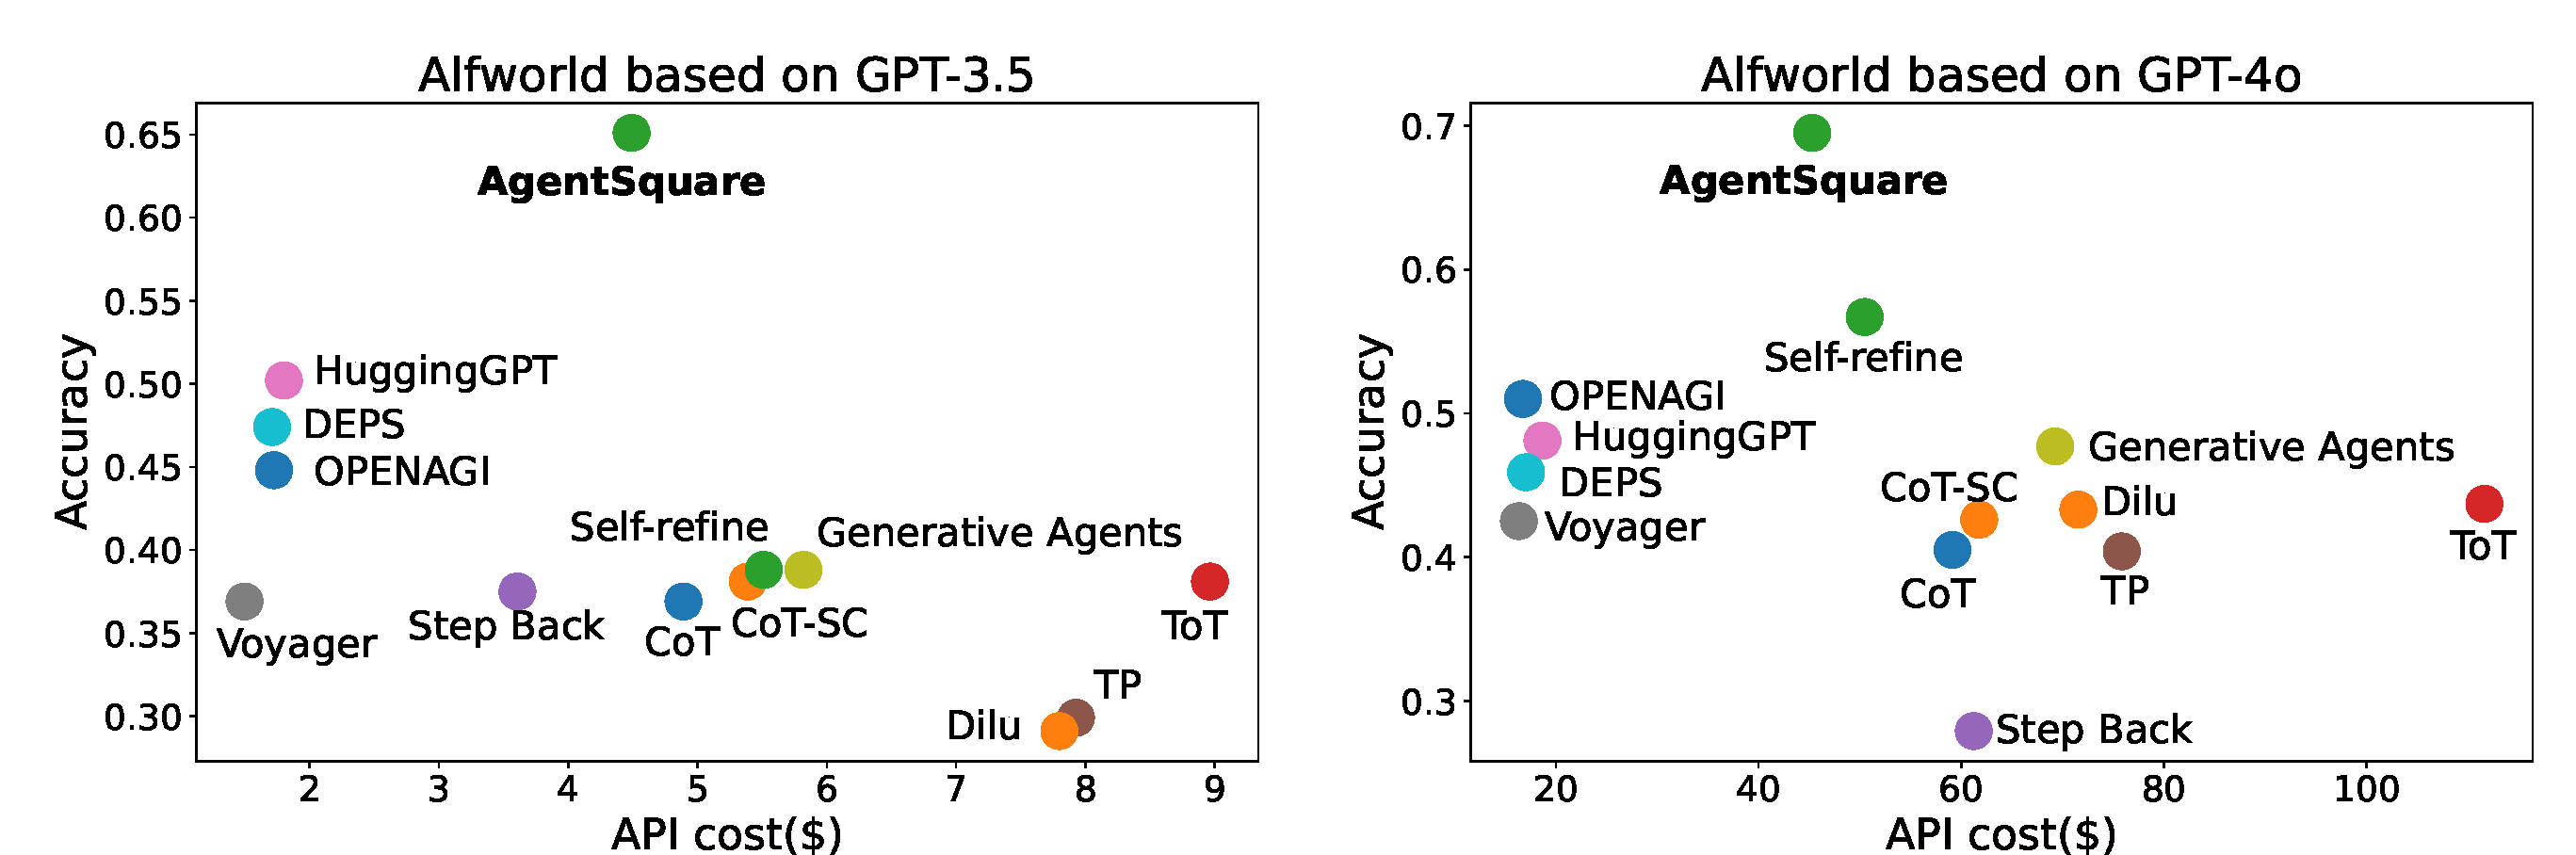
\includegraphics[width=\textwidth]{Figures/fig4_alfworld.pdf}
% \includegraphics[width=12.5cm]{Figures/f4(sci).pdf}
% \includegraphics[width=12.5cm]{Figures/f4(travel).pdf}
%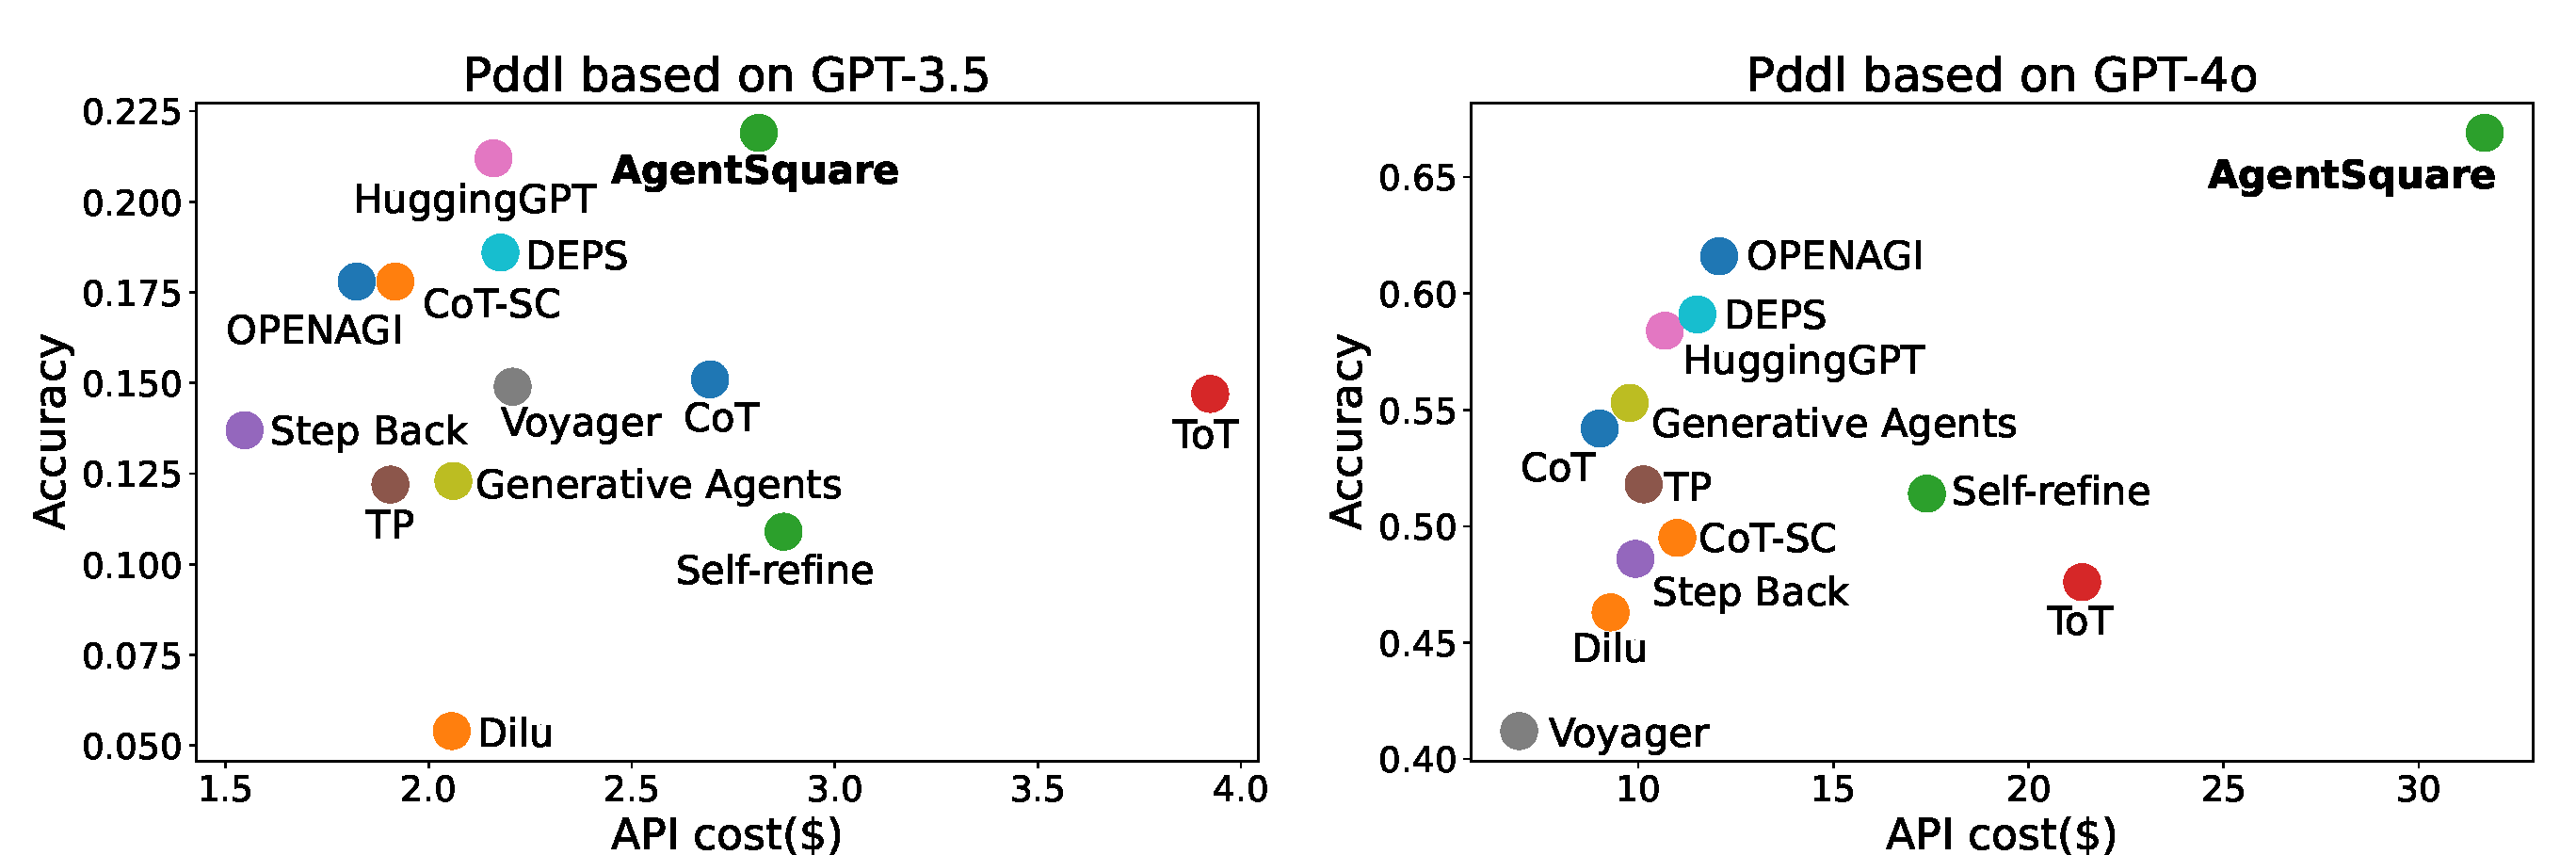
\includegraphics[width=12.5cm]{Figures/fig4_pddl.pdf}
\caption{Performance versus API costs visualization on ALFWorld task.}
\label{fig4:performance-cost}
\end{center}
\end{figure}

\begin{figure}[!t]
\begin{center}
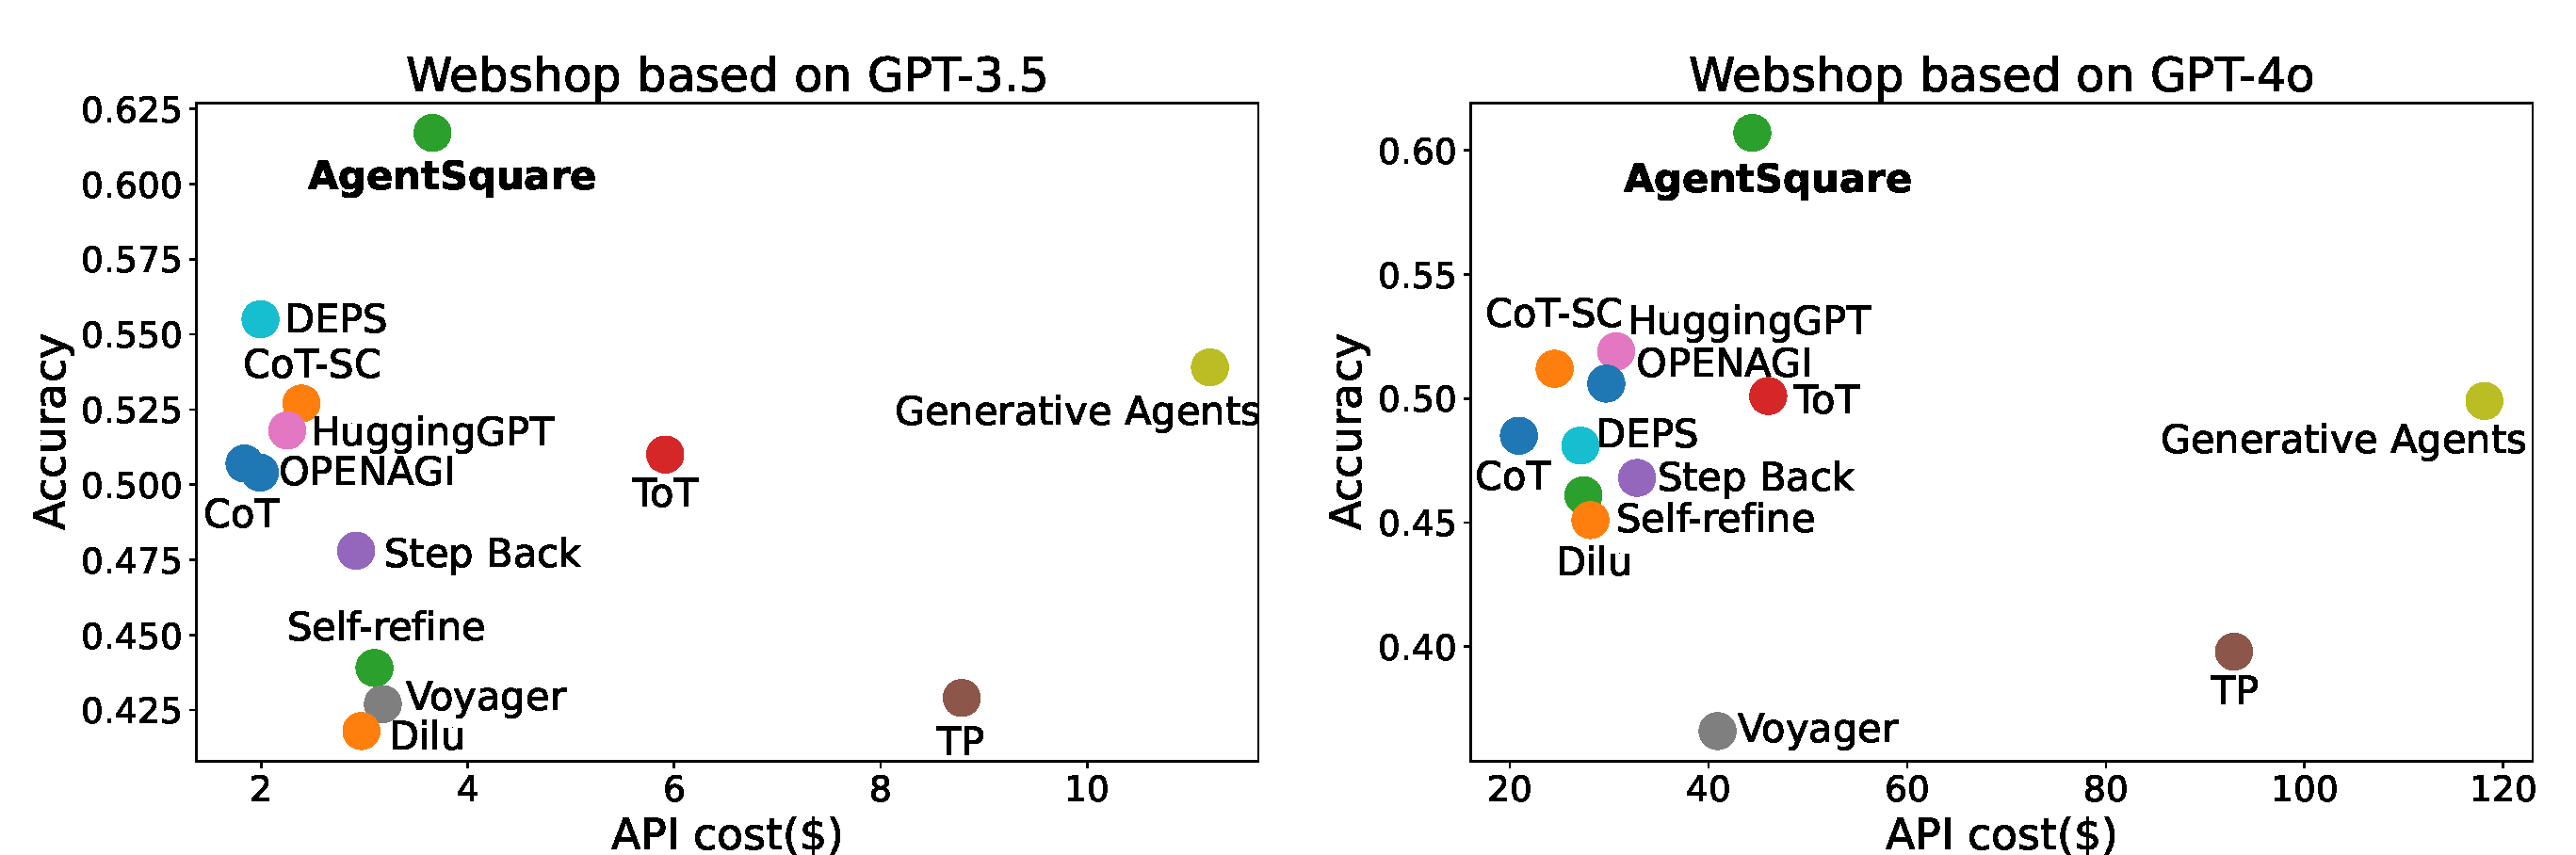
\includegraphics[width=\textwidth]{Figures/fig4_webshop.pdf}
\caption{Performance versus API costs visualization on Webshop.}
\label{app:performance-cost1}
\end{center}
\end{figure}

\begin{figure}[!t]
\begin{center}
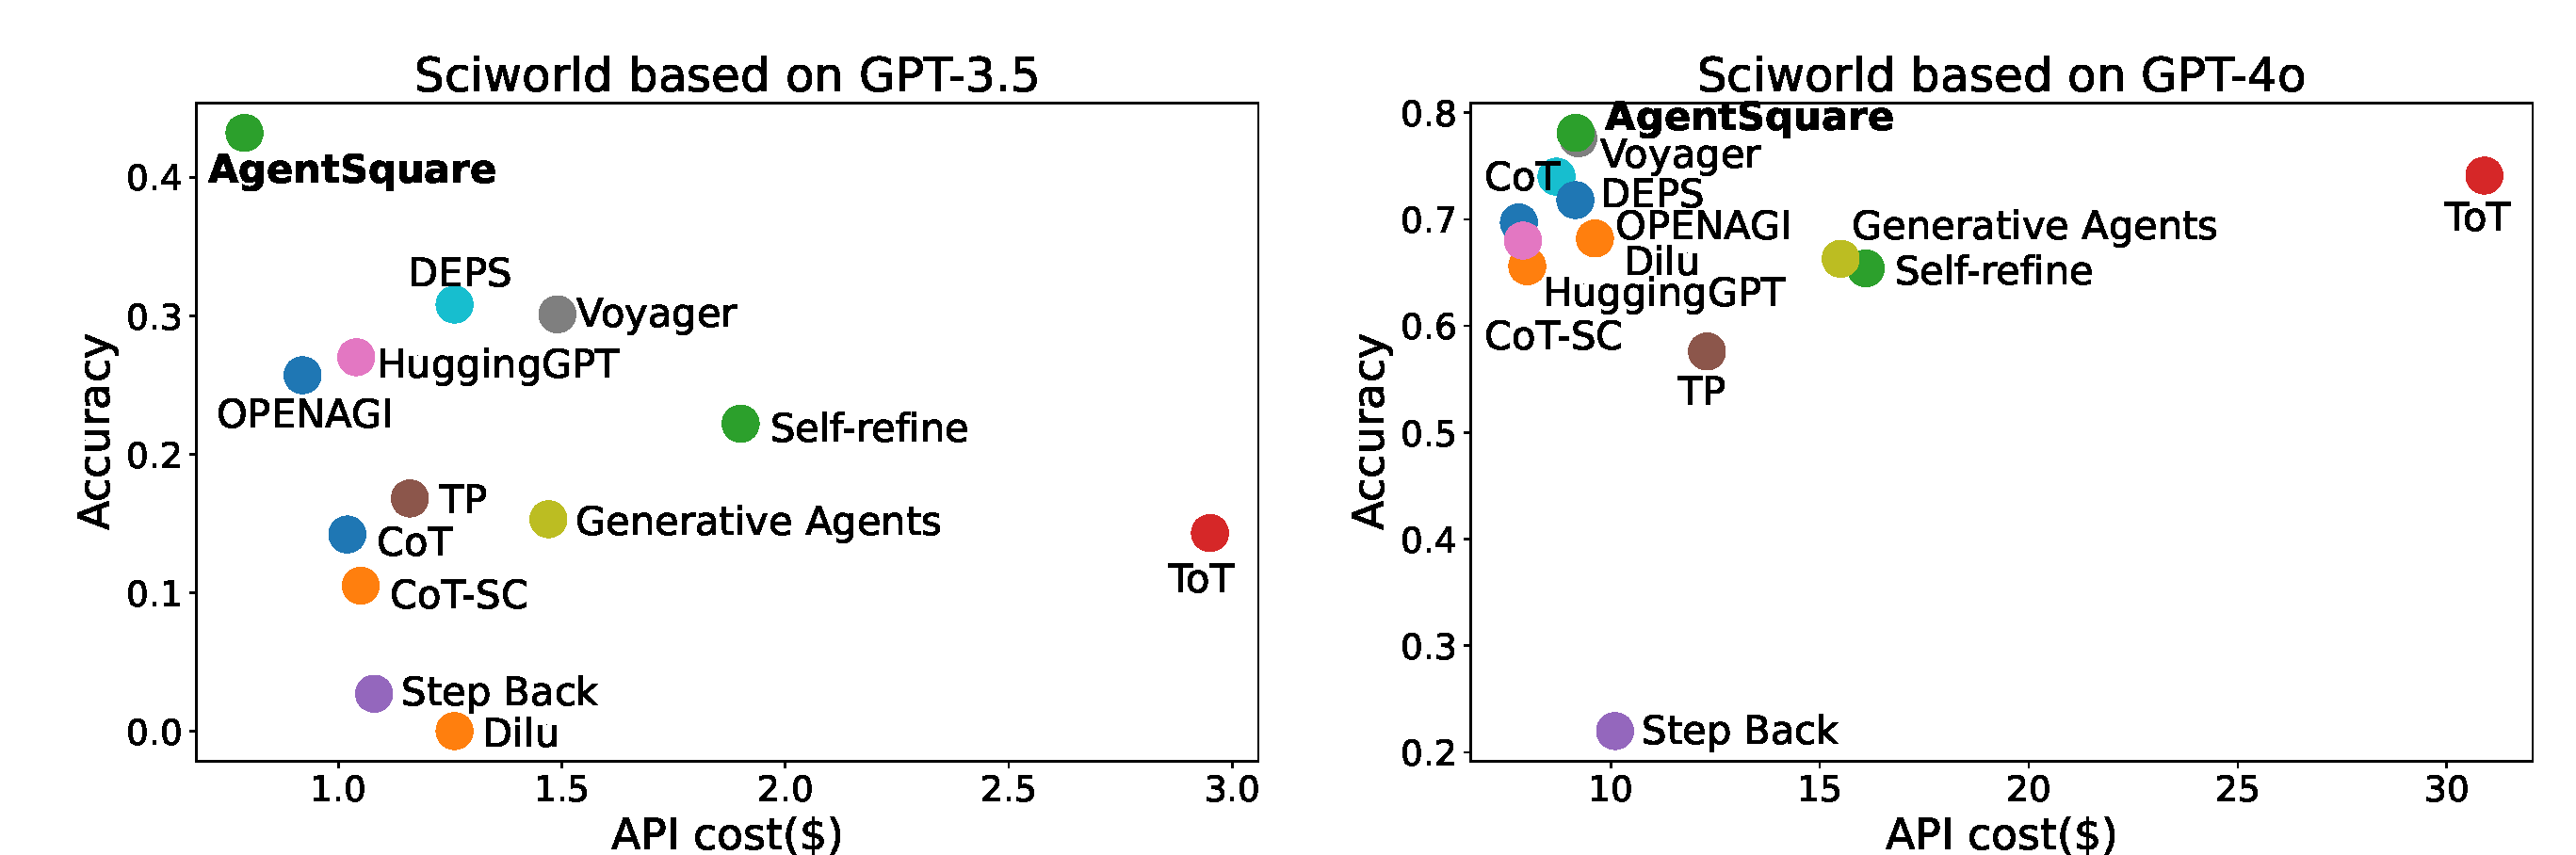
\includegraphics[width=\textwidth]{Figures/fig4_sciworld.pdf}
\caption{Performance versus API costs visualization on Sciworld.}
\label{app:performance-cost2}
\end{center}
\end{figure}

\begin{figure}[!t]
\begin{center}
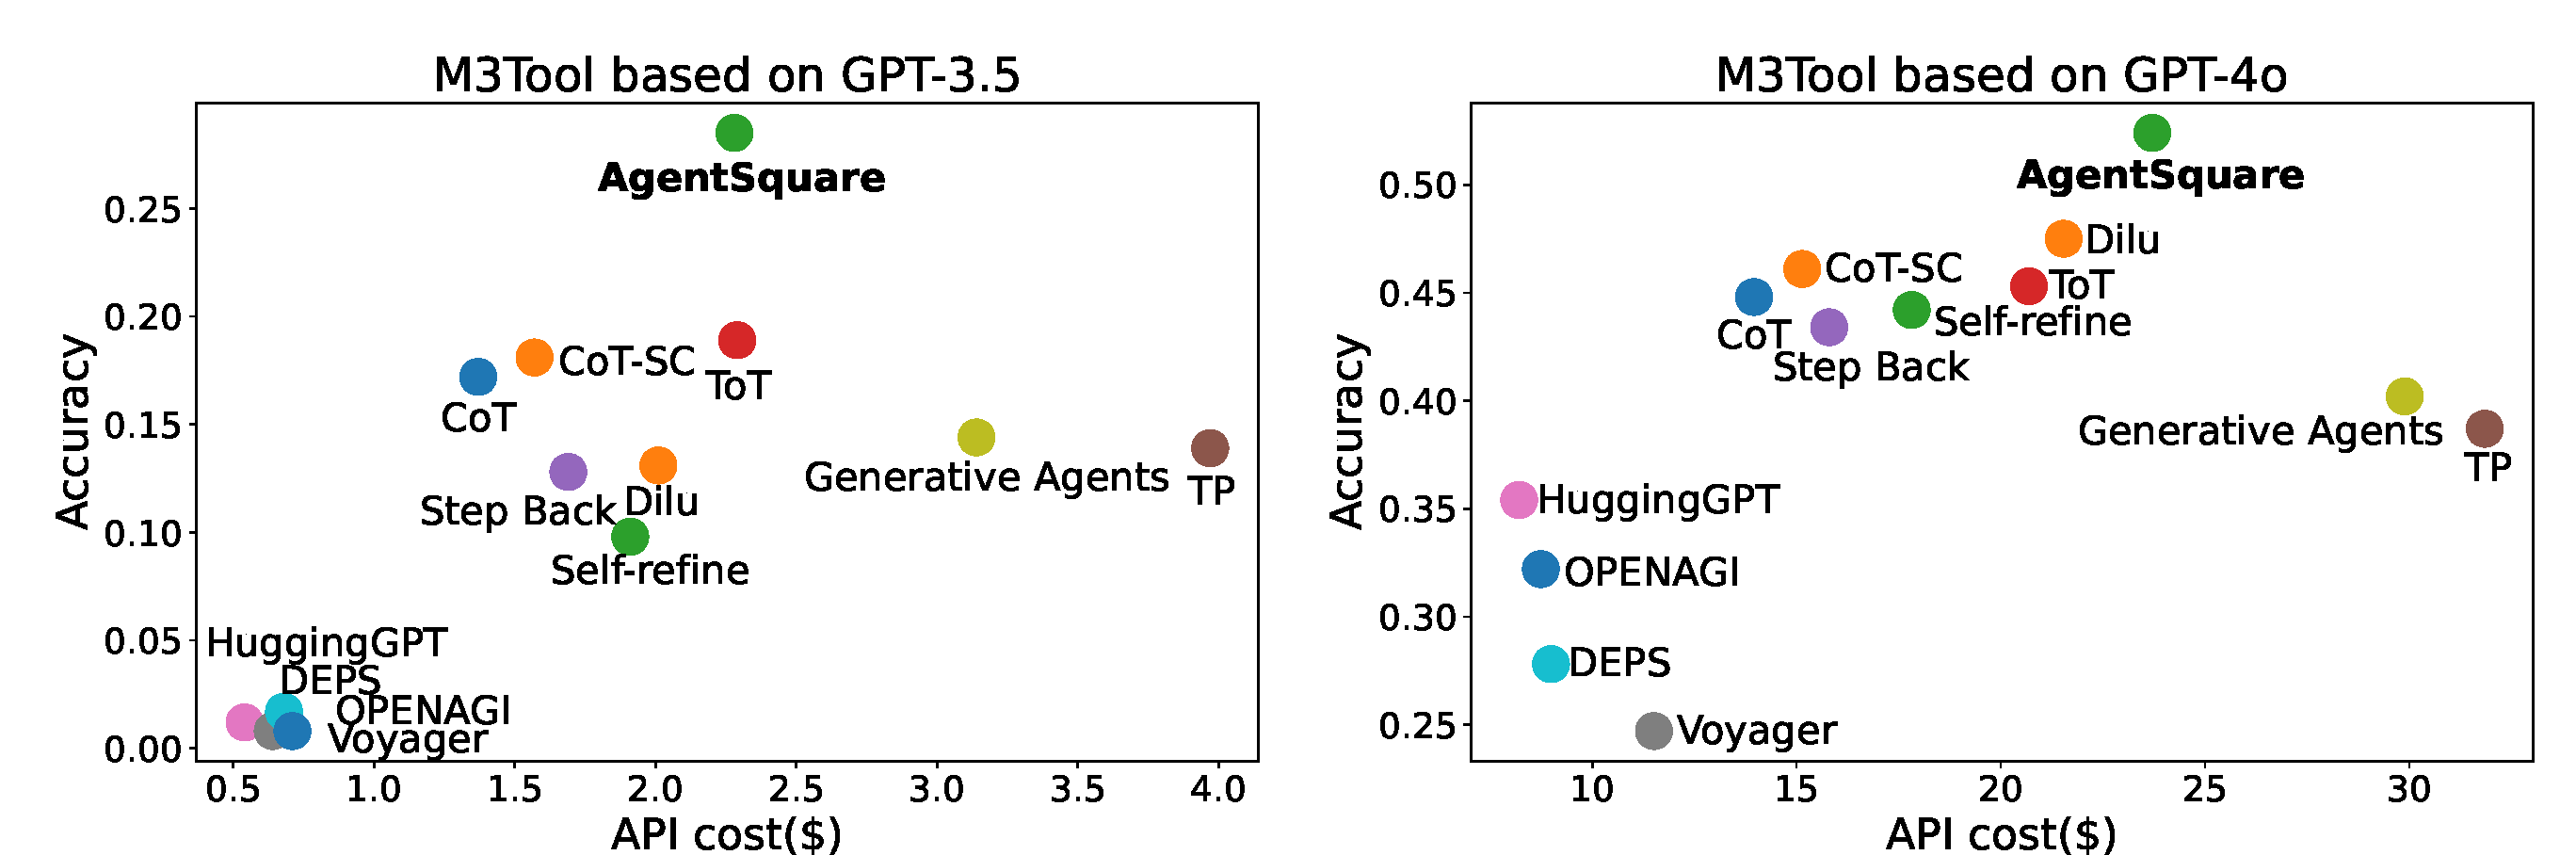
\includegraphics[width=\textwidth]{Figures/fig4_m3tool.pdf}
\caption{Performance versus API costs visualization on M3tool.}
\label{app:performance-cost3}
\end{center}
\end{figure}

\begin{figure}[!t]
\begin{center}
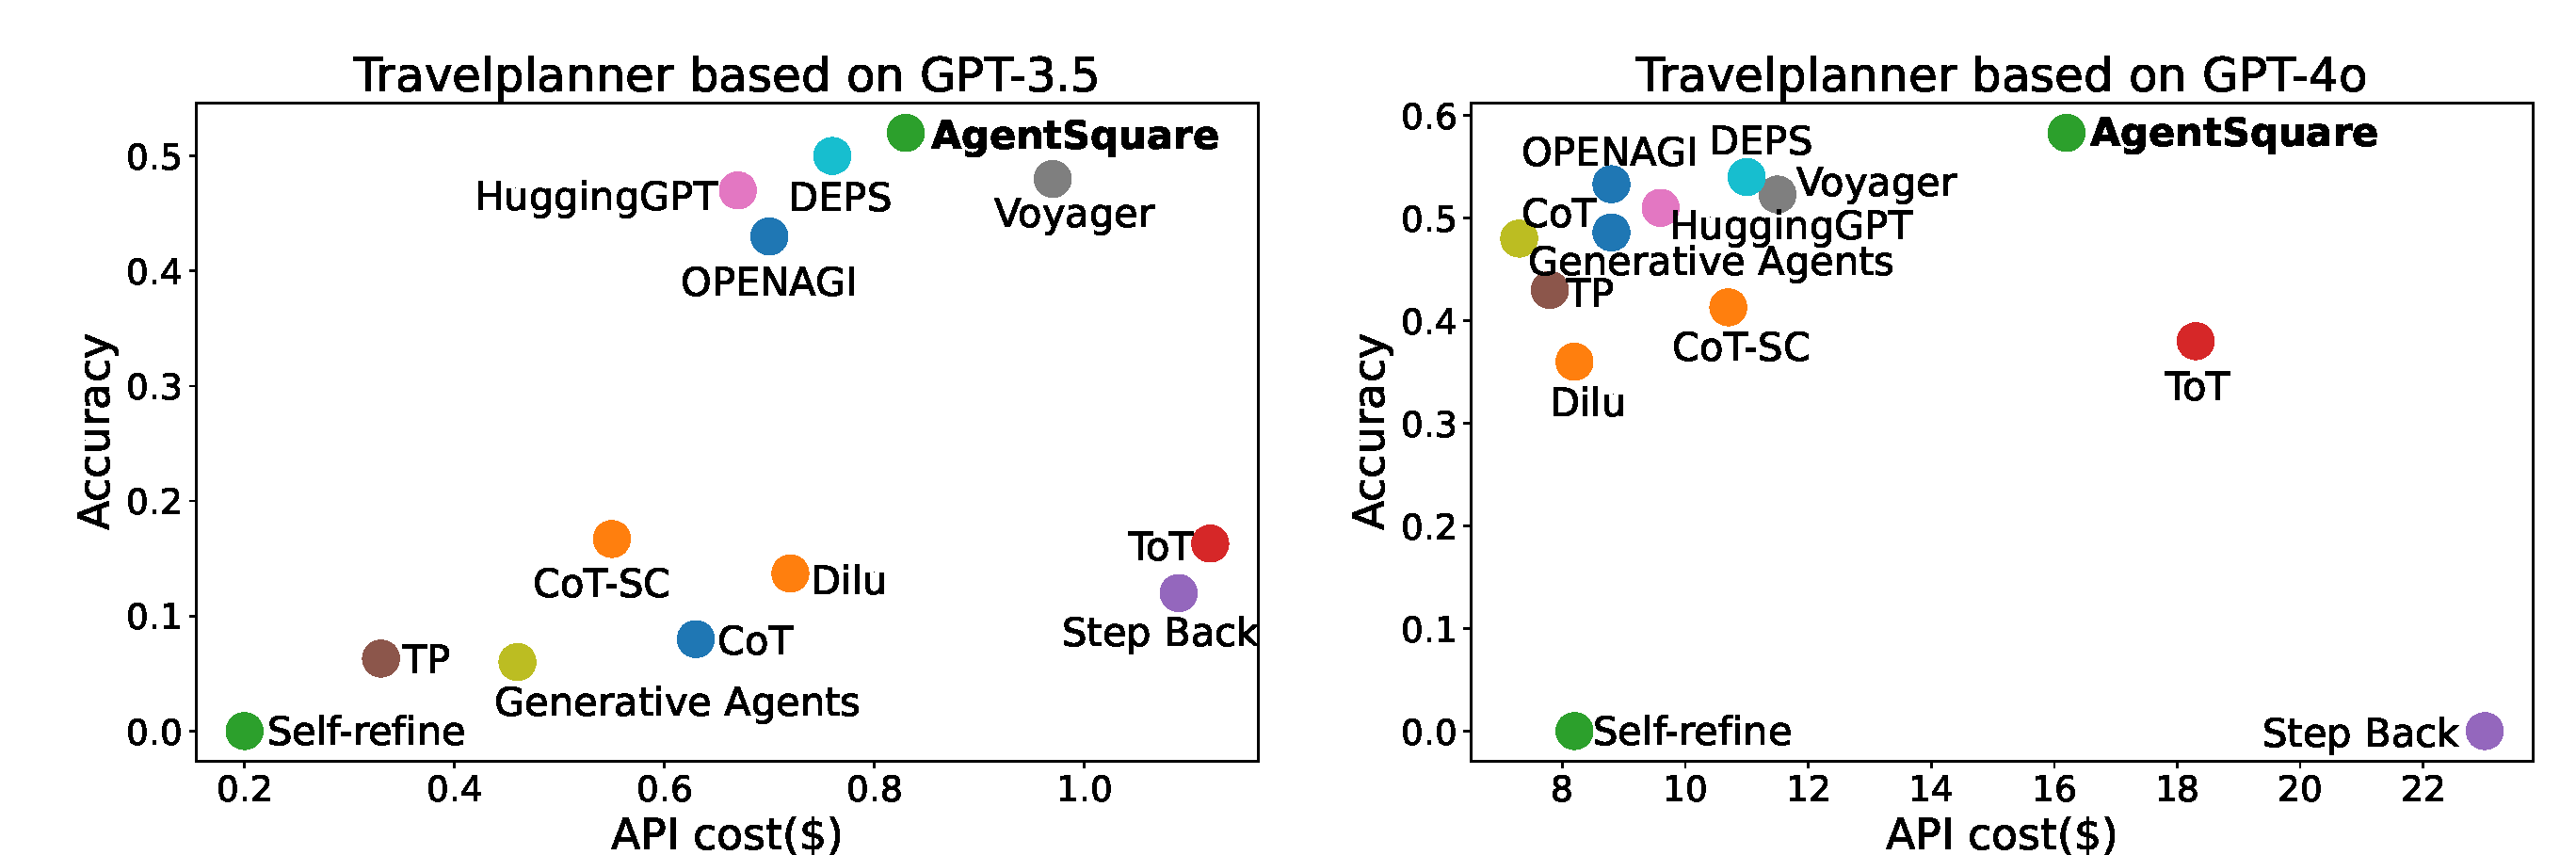
\includegraphics[width=\textwidth]{Figures/fig4_travelplanner.pdf}
\caption{Performance versus API costs visualization on Travelplanner.}
\label{app:performance-cost4}
\end{center}
\end{figure}

\begin{figure}[!t]
\begin{center}
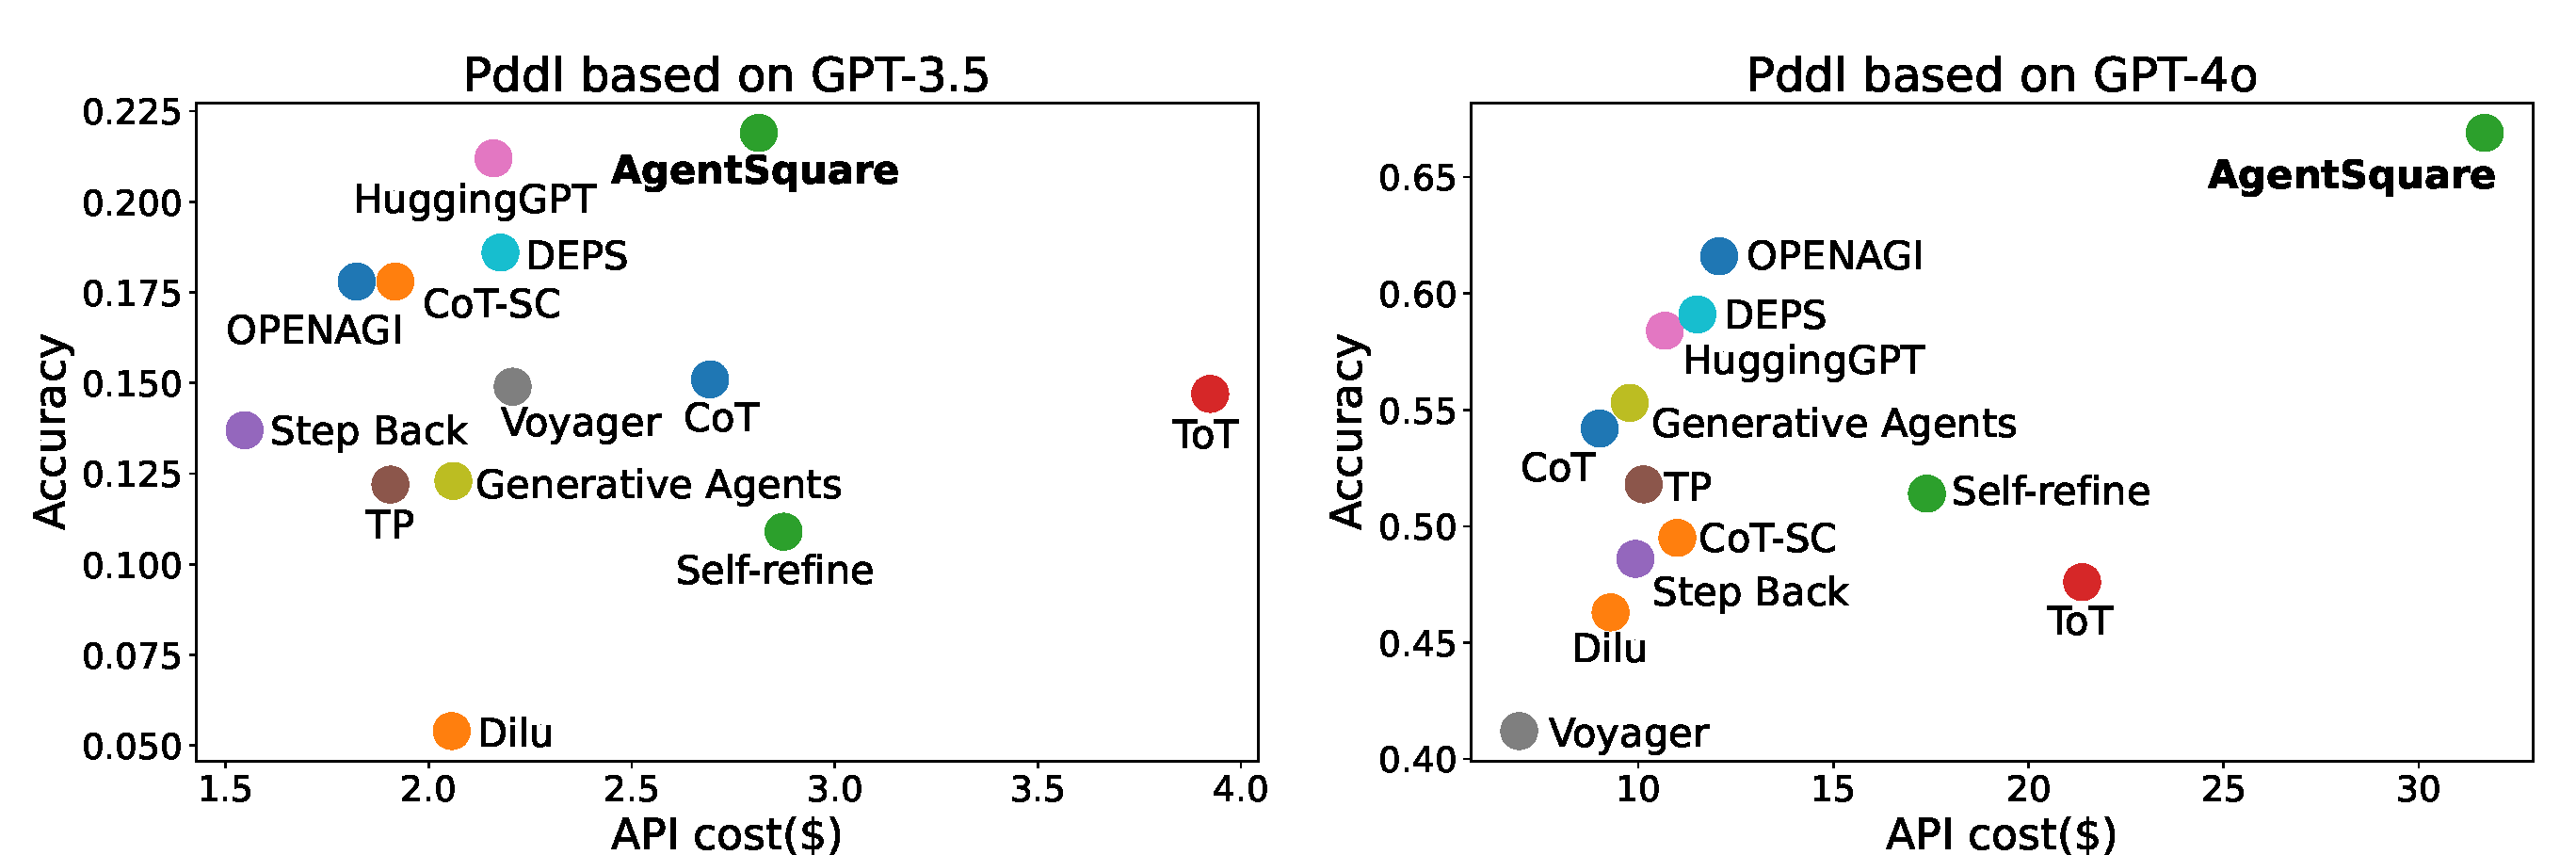
\includegraphics[width=\textwidth]{Figures/fig4_pddl.pdf}
\caption{Performance versus API costs visualization on PDDL.}
\label{app:performance-cost5}
\end{center}
\end{figure}

\begin{figure}[!t]
\begin{center}
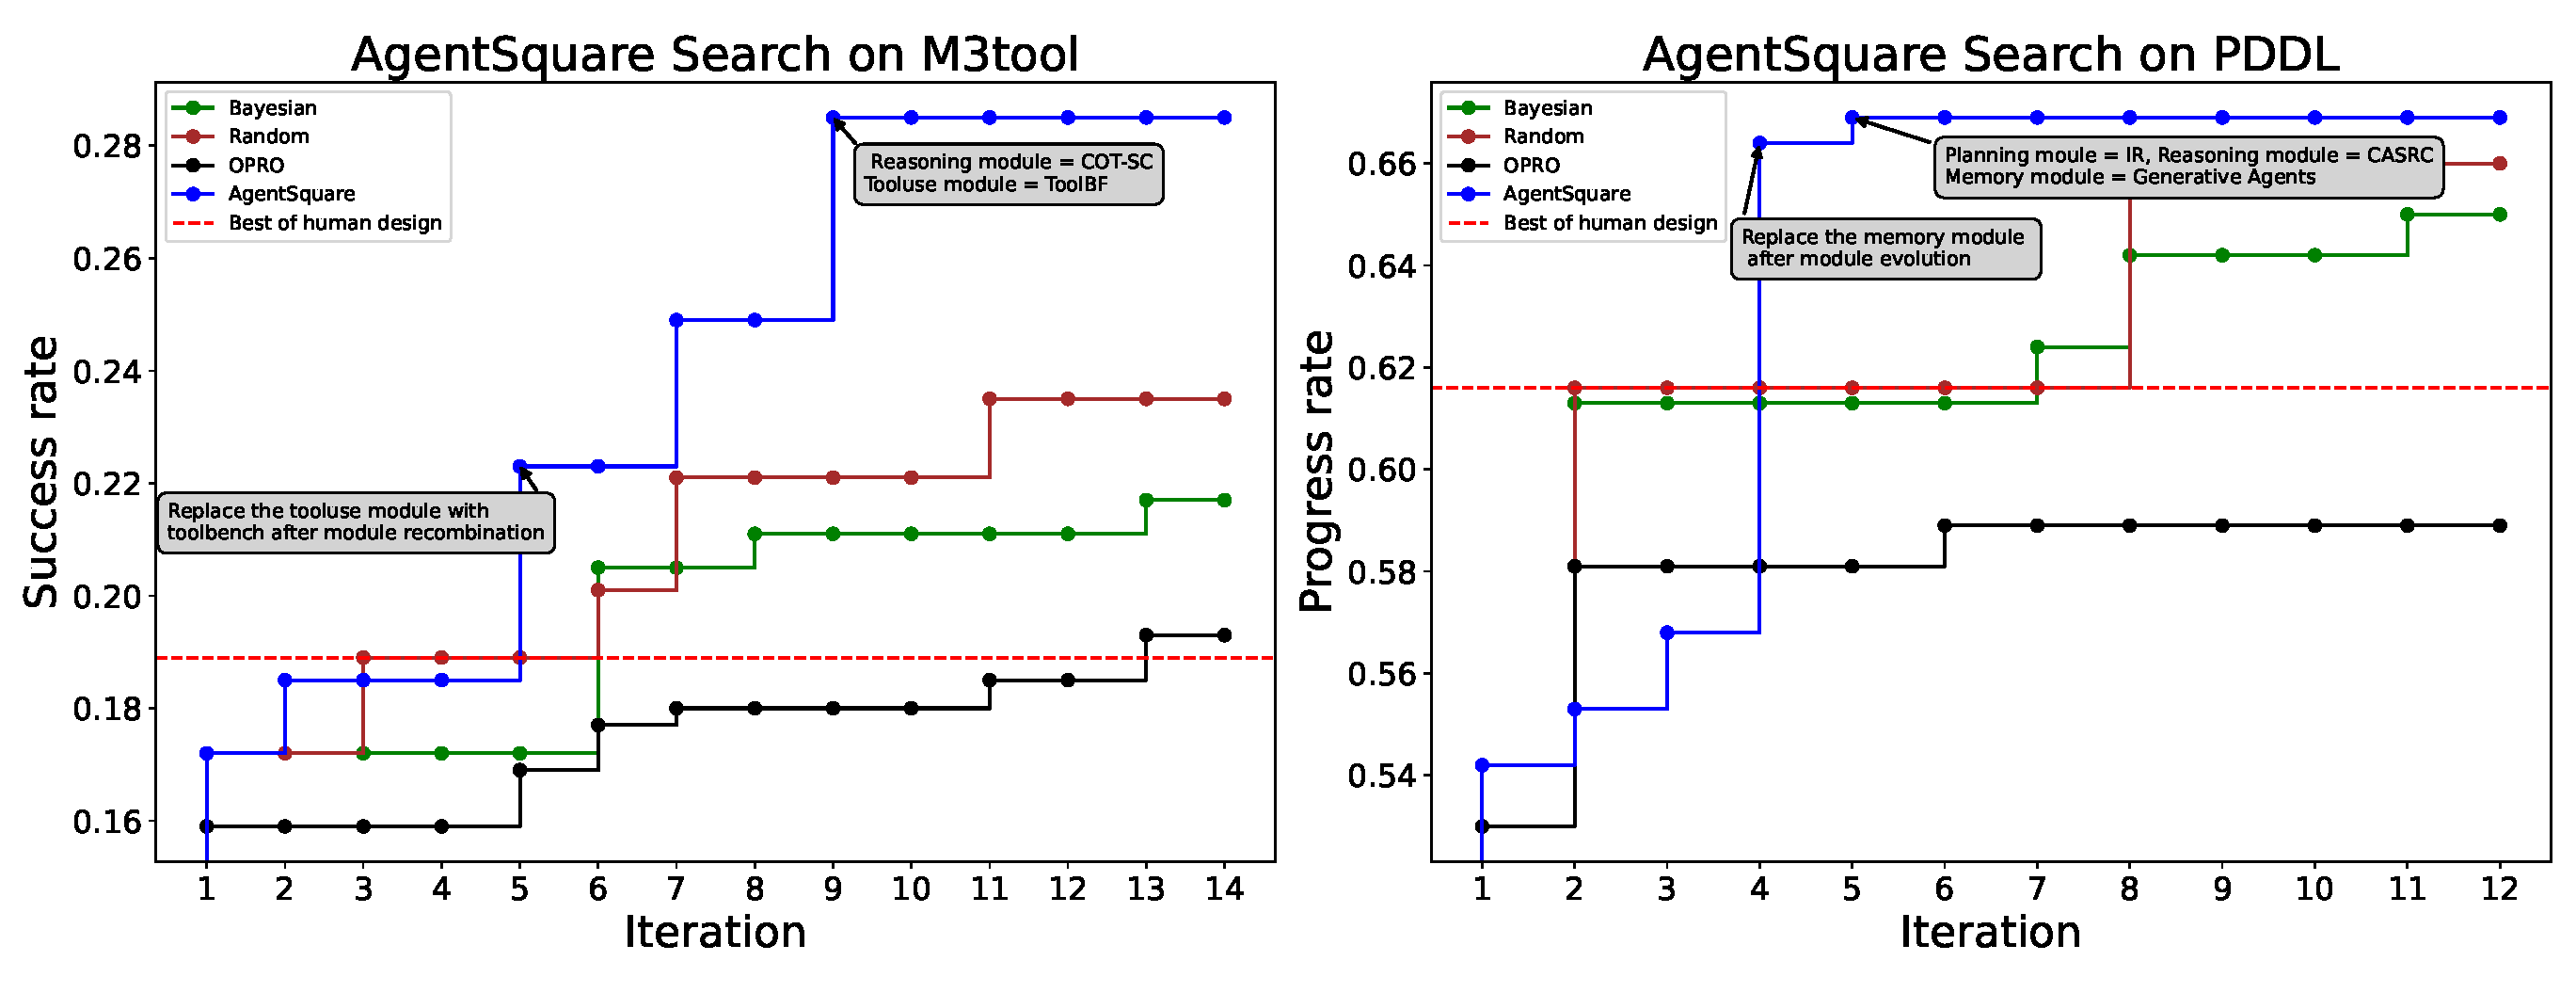
\includegraphics[width=\textwidth]{Figures/fig5_m3tool_pddl.pdf}
\caption{AgentSquare search trajectory on M3tool and PDDL (more hand-crafted agents, specific module combinations when surpassing best hand-crafted and the final evolved agent, other search baselines).}
\label{app:trajectory1}
\end{center}
\end{figure}

\begin{figure}[!t]
\begin{center}
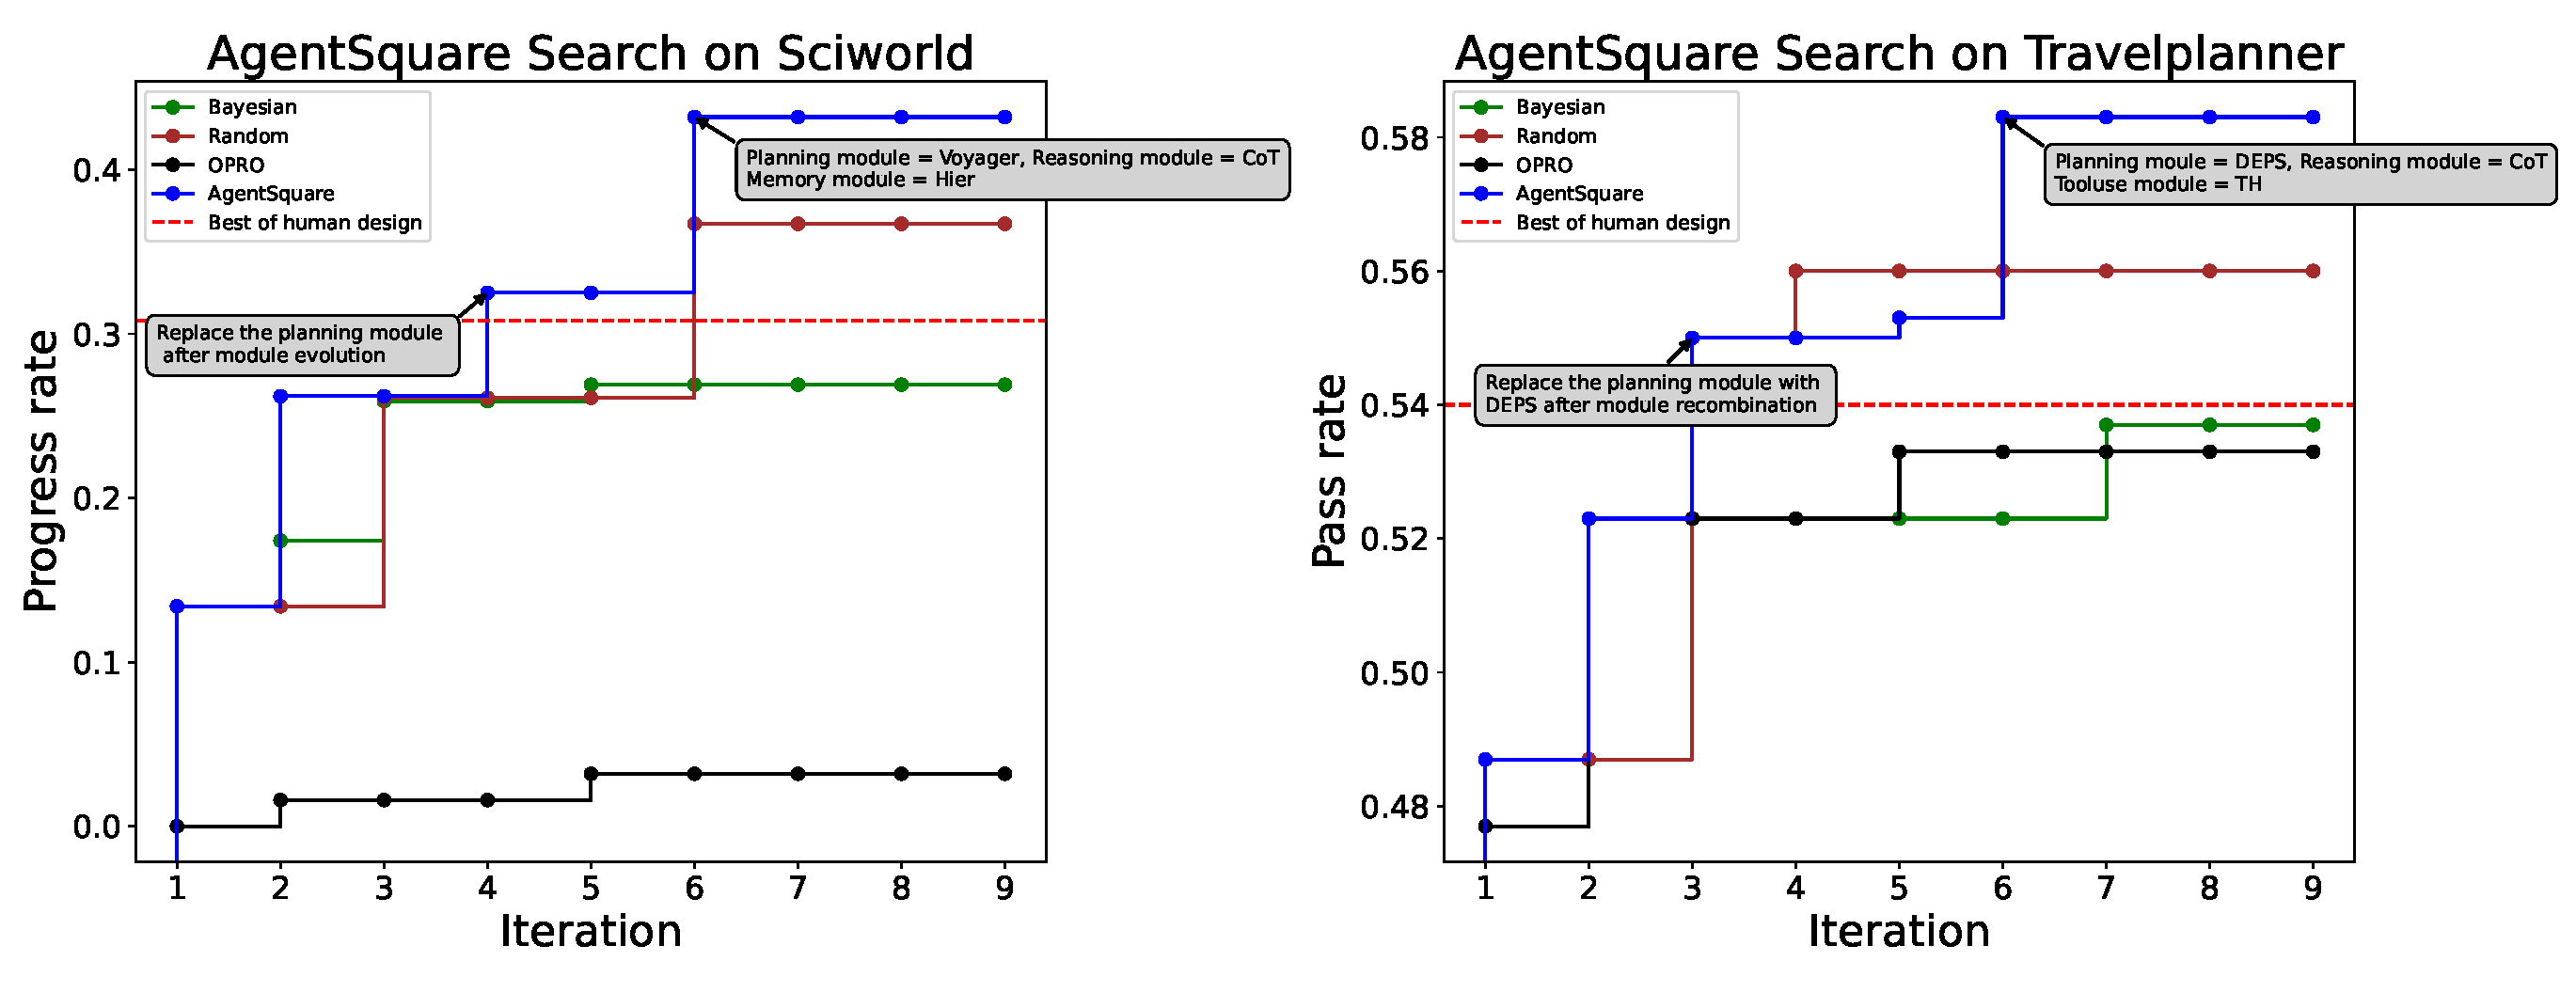
\includegraphics[width=\textwidth]{Figures/fig5_sciworld_travelplanner.pdf}
\caption{AgentSquare search trajectory on Sciworld and Travelplanner (more hand-crafted agents, specific module combinations when surpassing best hand-crafted and the final evolved agent, other search baselines).}
\label{app:trajectory2}
\end{center}
\end{figure}

\begin{figure}[!t]
\begin{center}
%\fbox{\rule[-.5cm]{0cm}{4cm} \rule[-.5cm]{4cm}{0cm}}
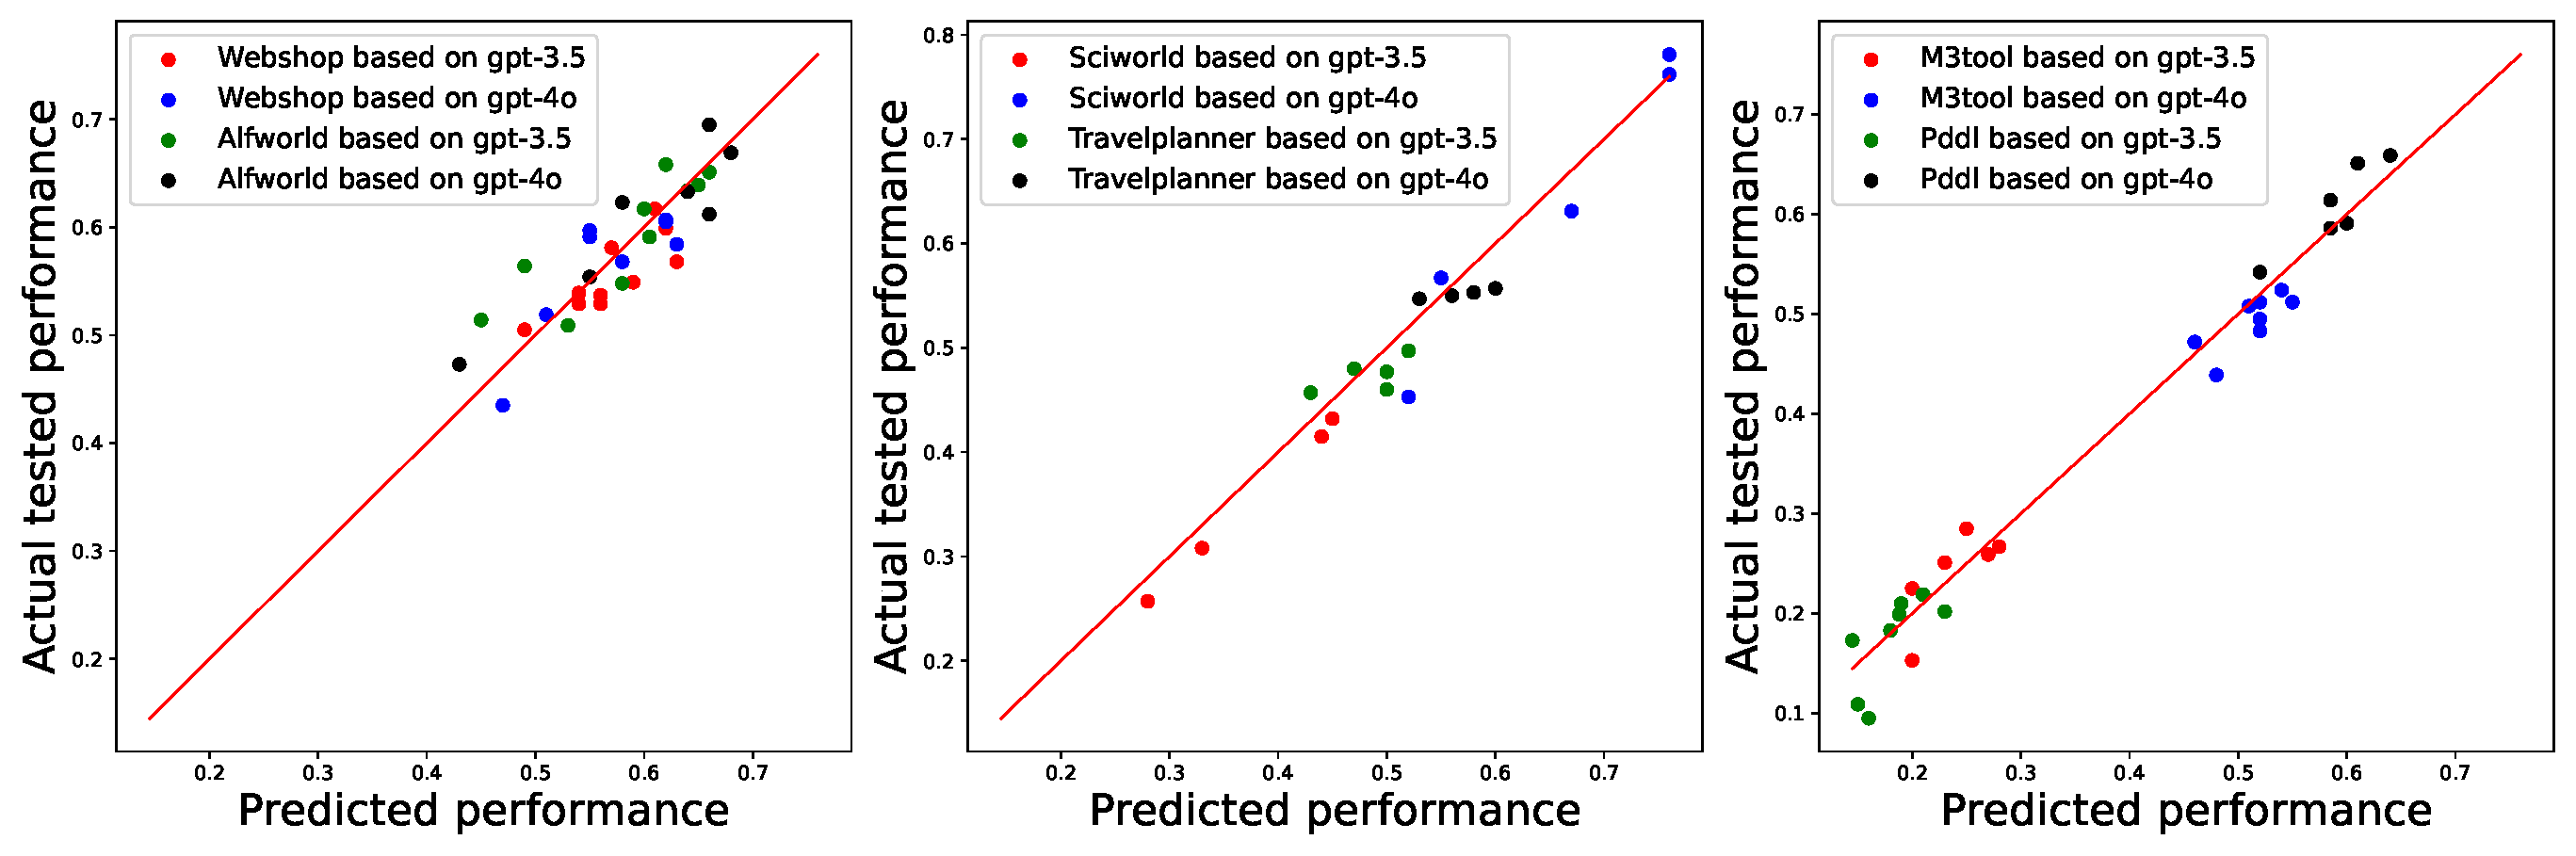
\includegraphics[width=0.85\textwidth]{Figures/fig5-more_data_points.pdf}
\caption{Validation of the effectiveness of the performance predictor on dynamically searched agents for each task.}
\label{pp-search}
\end{center}
\end{figure}

% \begin{figure}[h]
% \begin{center}
% 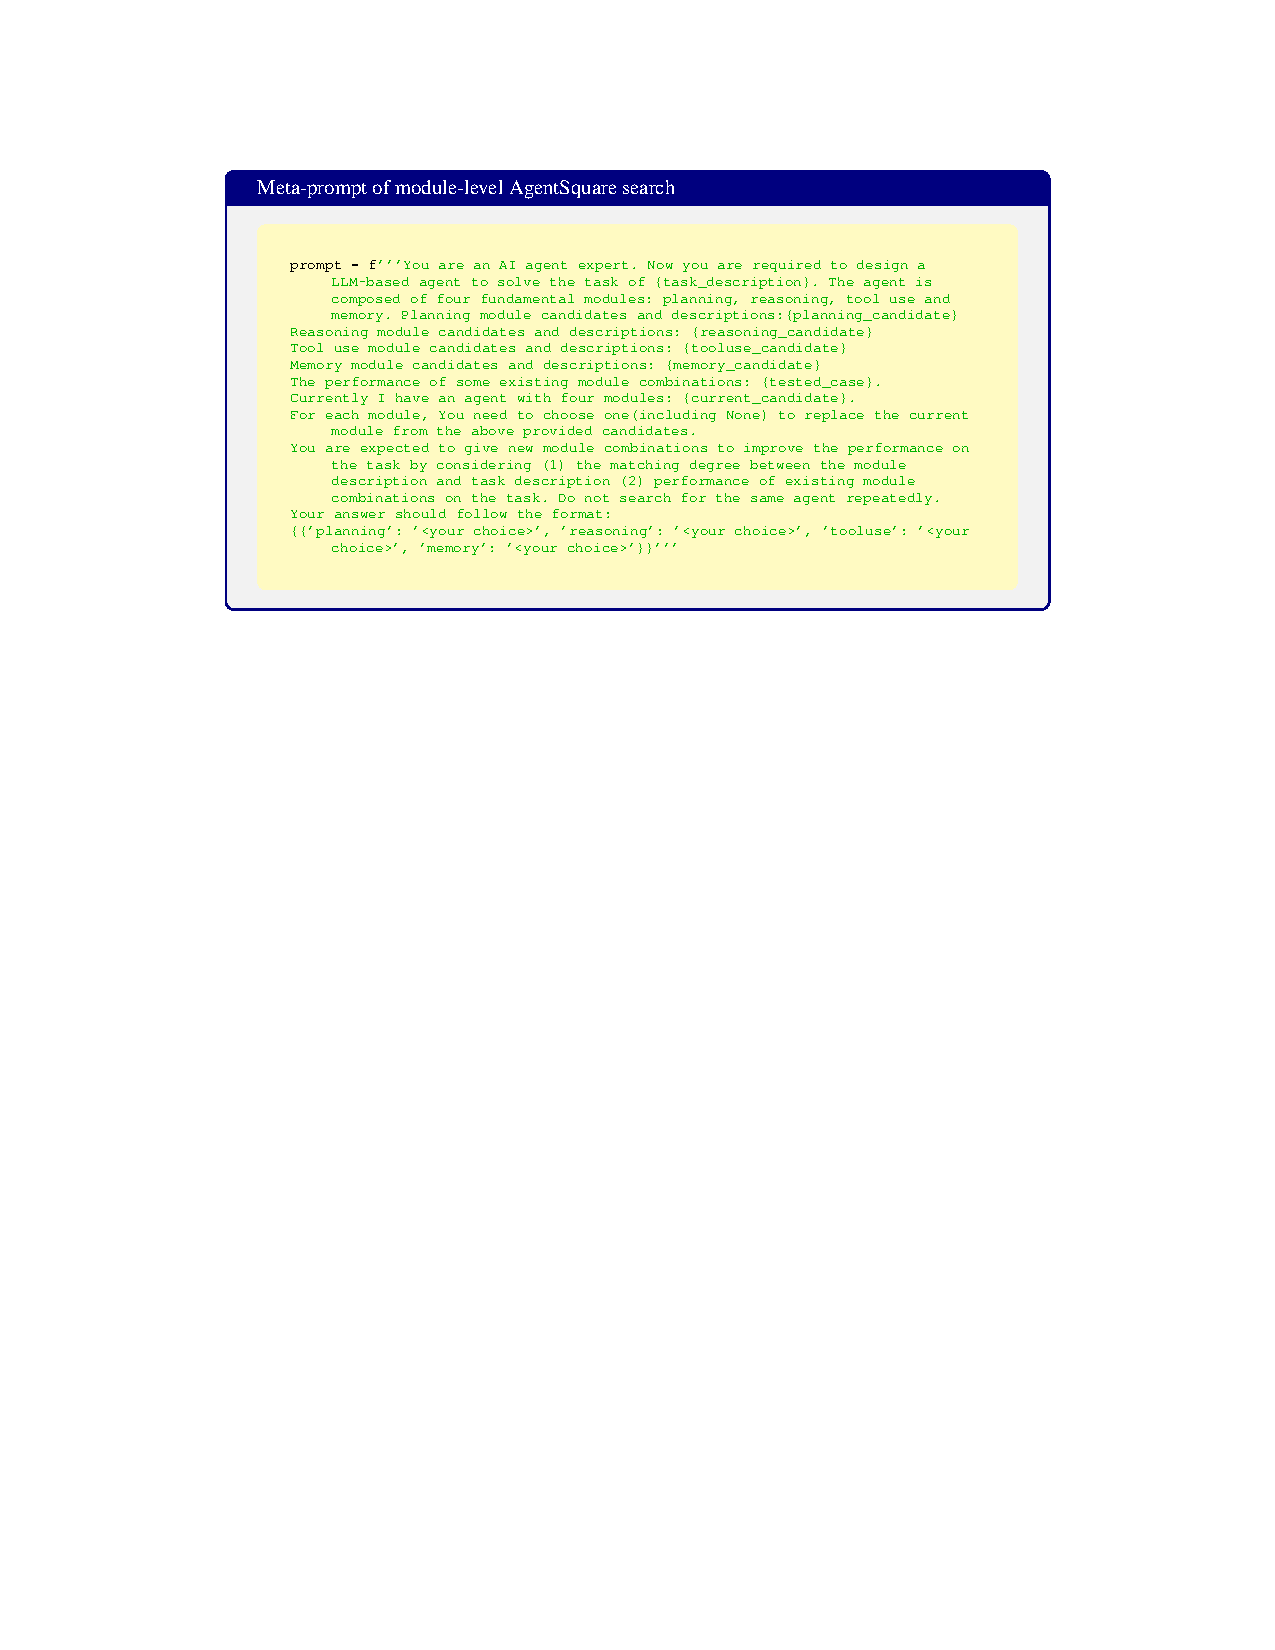
\includegraphics[width=\textwidth]{Figures/prompt_module_search.pdf}
% \caption{Meta-prompt of module recombination in AgentSquare search.}
% \label{app:module-level1}
% \end{center}
% \end{figure}

% \begin{figure}[h]
% \begin{center}
% 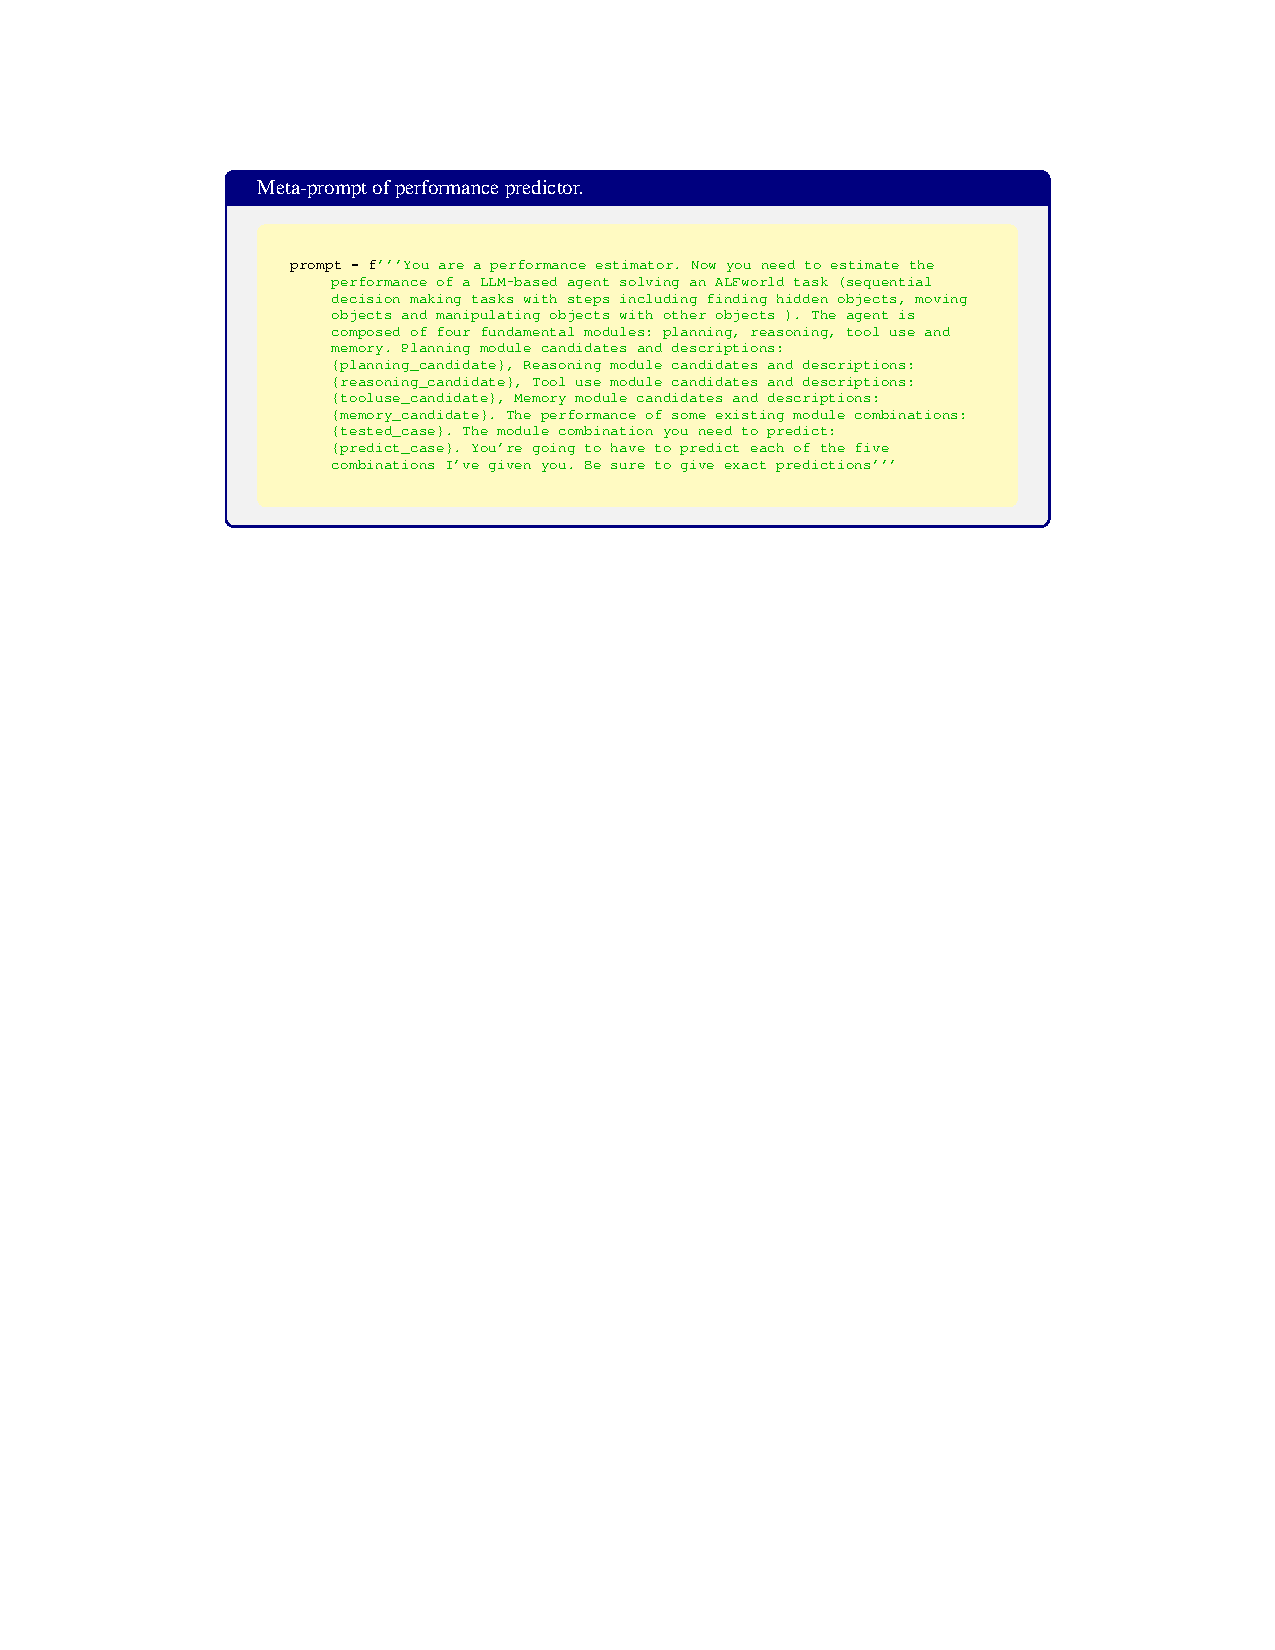
\includegraphics[width=\textwidth]{Figures/prompt_performance_predictor.pdf}
% \caption{Meta-prompt of performance predictor.}
% \label{app:pp-prompt}
% \end{center}
% \end{figure}

% \begin{figure}[h]
% \begin{center}
% 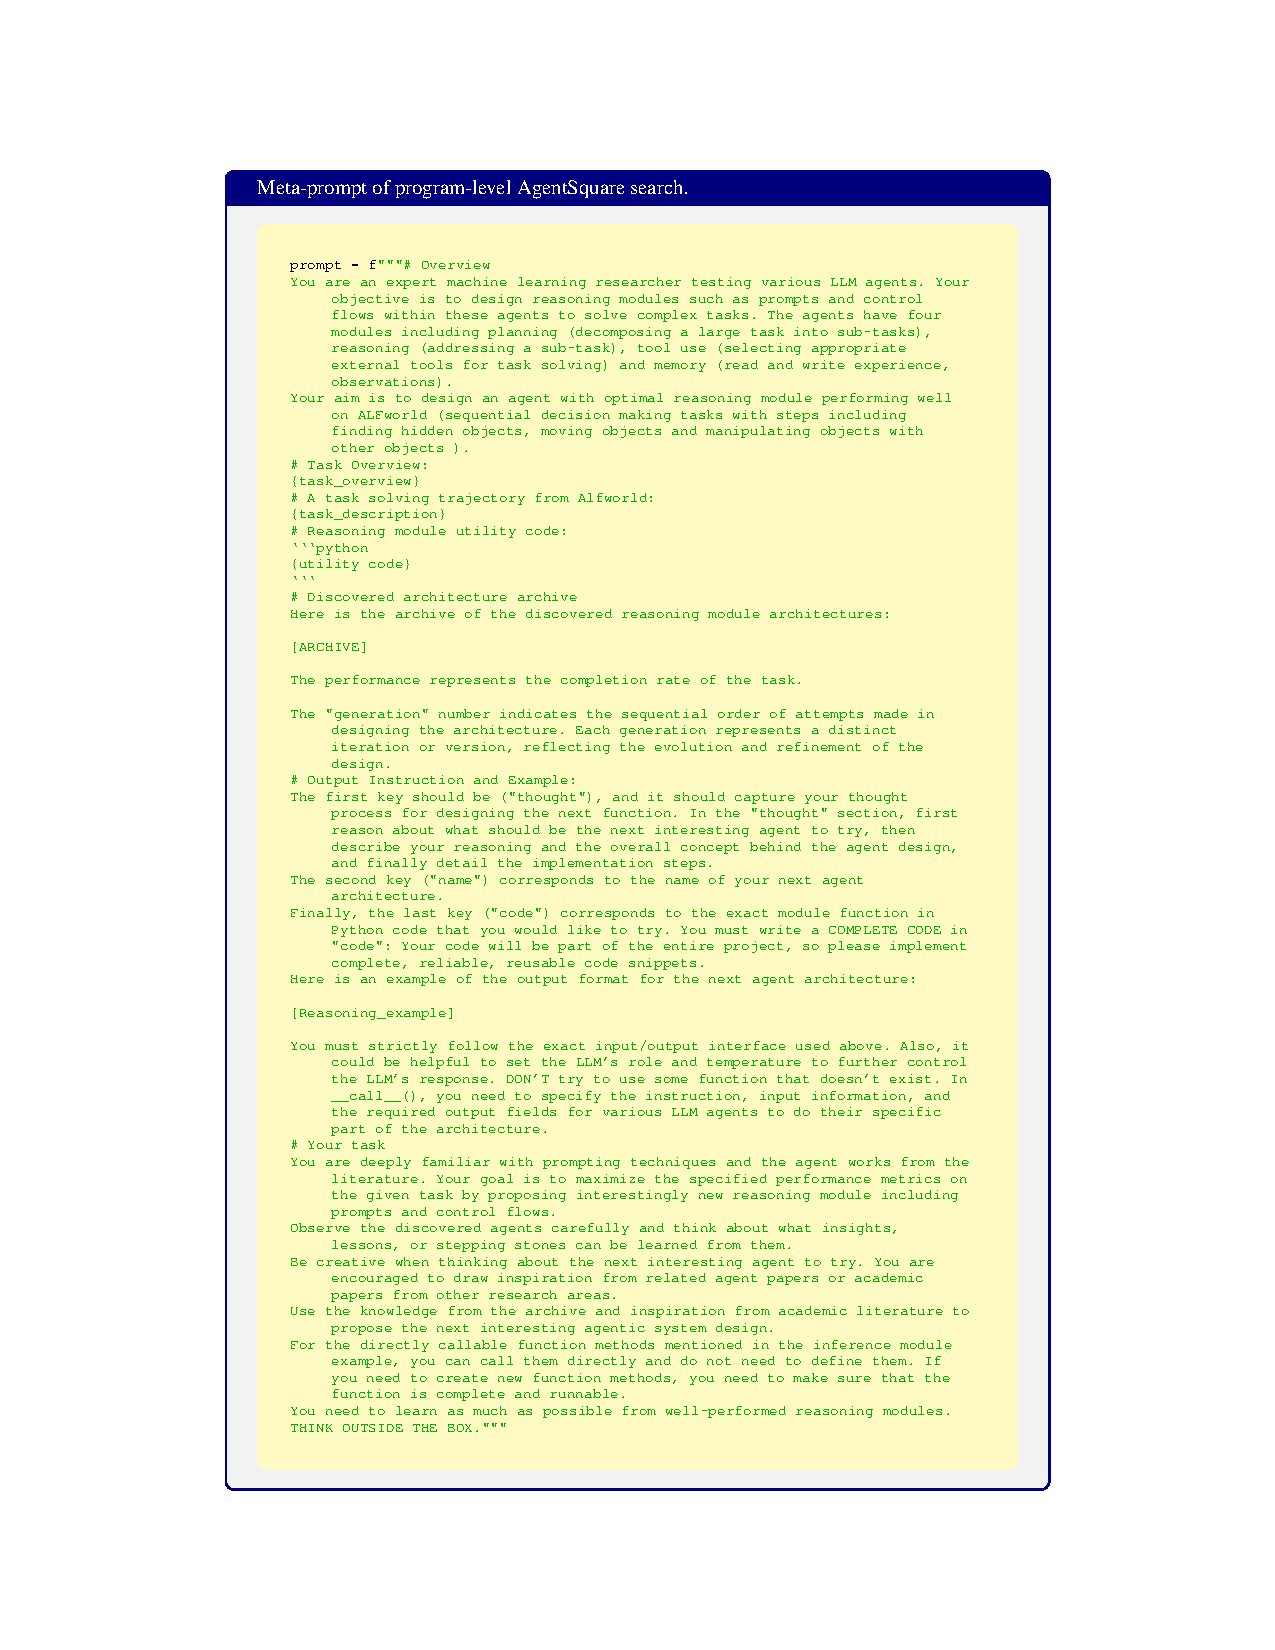
\includegraphics[width=0.9871\textwidth]{Figures/prompt_program_search.pdf}
% \caption{Meta-prompt of module evolution in AgentSquare search (partly refer to ADAS).}
% \label{app:prompt-level}
% \end{center}
% \end{figure}

% \newpage
% % 创建带有蓝色边框的框
% \begin{tcolorbox}[colback=gray!10, colframe=blue!50!black, title=Meta-prompt of module-level AgentSquare search]
% % 使用高亮的黄色背景色显示部分文本
% \begin{tcolorbox}[colback=yellow!30, colframe=yellow!30]
% \lstset{basicstyle=\scriptsize\ttfamily} % 调整左边距
% \begin{lstlisting}
% prompt = f'''You are an AI agent expert. Now you are required to design a LLM-based agent to solve the task of {task_description}. The agent is composed of four fundamental modules: planning, reasoning, tool use and memory. Planning module candidates and descriptions:{planning_candidate}
% Reasoning module candidates and descriptions: {reasoning_candidate}
% Tool use module candidates and descriptions: {tooluse_candidate}
% Memory module candidates and descriptions: {memory_candidate}
% The performance of some existing module combinations: {tested_case}.
% Currently I have an agent with four modules: {current_candidate}.
% For each module, You need to choose one(including None) to replace the current module from the above provided candidates.
% You are expected to give new module combinations to improve the performance on the task by considering (1) the matching degree between the module description and task description (2) performance of existing module combinations on the task. Do not search for the same agent repeatedly.
% Your answer should follow the format:
% {{'planning': '<your choice>', 'reasoning': '<your choice>', 'tooluse': '<your choice>', 'memory': '<your choice>'}}'''
% \end{lstlisting}
% \end{tcolorbox}
% \end{tcolorbox}


% \newpage
% % 创建带有蓝色边框的框
% \begin{tcolorbox}[colback=gray!10, colframe=blue!50!black, title=HTSS]

% \textbf{Insights:} Observing the current performance of the reasoning modules, it seems that techniques like Chain-of-Thought (CoT) and Tree-of-Thoughts (ToT) have offered improvements by breaking down the task into smaller steps and evaluating multiple reasoning paths. The Self-Consistency (SC) approach also shows promise by generating multiple answers and voting on them, while the Self-Refine module uses iterative improvement based on feedback.\\
% \textbf{Overall Idea:} To further enhance the performance, we can integrate a combination of these techniques into a single module. Specifically, we can combine the Tree-of-Thoughts (ToT) approach with Self-Consistency (SC) and Self-Refine. This combined approach would involve generating multiple reasoning paths, evaluating them to choose the best path, and then iteratively refining the chosen path based on feedback.\\
% \textbf{Implementation:} 1. Generate Multiple Reasoning Paths: Use the Tree-of-Thoughts (ToT) approach to generate multiple reasoning paths.2. Evaluate and Choose the Best Path: Use Self-Consistency (SC) to evaluate these paths by voting and selecting the most common or accurate path.3. Refine the Chosen Path: Use Self-Refine to iteratively improve the chosen path based on feedback.4. Prompt Structure: Craft prompts that encourage step-by-step problem-solving, refer to similar solved examples, and refine output based on feedback.
% % 使用高亮的黄色背景色显示部分文本
% \begin{tcolorbox}[colback=yellow!30, colframe=yellow!30]
% \lstset{basicstyle=\scriptsize\ttfamily} % 调整左边距
% \begin{lstlisting}
% class REASONING_HYBRID_TOT_SC_SELFREFINE():
%     def __init__(self, profile_type_prompt, memory, tooluse, llms_type):
%         self.feedback = ''
%         self.profile_type_prompt = profile_type_prompt
%         self.memory = memory
%         self.llm_type = llms_type[0]
%         self.tooluse = tooluse
%     def __call__(self, task_description: str, tool_instruction :str='', feedback :str= ''):
%         task_name = re.findall(r'Instruction:\s+(.*?)\s+\[Search\]', task_description)        
%         if self.memory is not None:
%             self.task_name_cache = task_name[1]
%             self.memory_cache = self.memory(task_description)
%             if task_description.count('Reasoning') == 2:
%                 self.memory_cache = self.memory_cache.split('Observation')[0]
%             elif task_description.count('Reasoning') == 4:
%                 self.memory_cache = 'Observation'.join(self.memory_cache.split('Observation')[0:3])
%             else:
%                 self.memory_cache = self.memory_cache
%         else:
%             self.memory_cache = ''
%         if self.tooluse is not None:
%             tooluse = self.tooluse(task_description, tool_instruction)
%         else:
%             tooluse = ''
%         split_text = task_description.rsplit('WebShop', 1)
%         examples = split_text[0]
%         task_description = 'WebShop' + split_text[1]
%         prompt = '''{tooluse}Solve the task step by step. Your output must follow the examples process. Don't refine your search. You have to choose one from a list of items.
% {memory}{examples}
% {task_description}'''
%         prompt = prompt.format(task_description=task_description, examples=examples, memory=self.memory_cache, tooluse=tooluse)
%         reasoning_results = llm_response(prompt=prompt, model=self.llm_type, temperature=0.1, stop_strs=['\n'], n=3)
%         # Evaluate and choose the best path
%         from collections import Counter
%         string_counts = Counter(reasoning_results)
%         best_path = string_counts.most_common(1)[0][0]
%         # Refine the chosen path based on feedback
%         refined_result = self.refine(best_path)
%         #reasoning_result = self.refine(reasoning_result)
%         return refined_result
% \end{lstlisting}
% \end{tcolorbox}
% \end{tcolorbox}

% \newpage
% % 创建带有蓝色边框的框
% \begin{tcolorbox}[colback=gray!10, colframe=blue!50!black, title=ToolBF]

% \textbf{Insights:} The previously discovered architectures indicate that leveraging multiple interactions or multiple attempts to identify the most suitable tool can enhance performance (as in Toolformer). Additionally, using a vector similarity approach to retrieve the most relevant tools (as in Toolbench) seems promising. \\
% \textbf{Overall Idea:} I propose combining the vector similarity approach with multiple attempts to maximize the chances of selecting the optimal tool. Specifically, I will augment the Toolbench approach by making multiple calls to the LLM to generate several potential solutions and then selecting the best one through a voting mechanism. \\
% \textbf{Implementation:} The implementation will involve converting instructions and API documentation into vector representations, retrieving the most relevant APIs, generating multiple responses using the LLM, and finally selecting the best response using a voting mechanism.
% % 使用高亮的黄色背景色显示部分文本
% \begin{tcolorbox}[colback=yellow!30, colframe=yellow!30]
% \lstset{basicstyle=\scriptsize\ttfamily} % 调整左边距
% \begin{lstlisting}
% class TOOLUSE_TOOLBENCHFORMER():
%     def __init__(self, llms_type):
%         self.llm_type = llms_type[0]
%         self.scenario_memory = {}
%         for name, tools in tooluse_IO_pool.items():
%             db_path = os.path.join('./db', f'api_pool{name}/') 
%             self.embedding = OpenAIEmbeddings()       
%             self.scenario_memory[name] = Chroma(
%                 embedding_function=self.embedding,
%                 persist_directory=db_path)
%             api_pattern = re.compile(r"\[(\d+)\] ([^:]+): (.+?)(?=\[\d+\]|\Z)", re.DOTALL)
%             api_matches = api_pattern.findall(tools)
%             documents = []
%             for match in api_matches:
%                 api_id, api_name, api_description = match     
%                 first_sentence = api_description.split('.')[0].strip() + '.'
%                 full_description = f"[{api_id}] {api_name}: {api_description.strip()}"
%                 doc = Document(
%                     page_content=first_sentence,
%                     metadata={
%                         "name": api_name.strip(),
%                         "description": full_description})
%                 documents.append(doc)
%             self.scenario_memory[name].add_documents(documents)
%     def __call__(self, task_description, tool_instruction, feedback_of_previous_tools):
%         similarity_results = self.scenario_memory[task_description].
%          similarity_search_with_score(tool_instruction, k=4)
%         tool_pool = []
%         for idx in range(0, len(similarity_results)):
%             tool_pool.append(similarity_results[idx][0].metadata['description'])
%         prompt = f'''
% You have access to the following tools:
% {tool_pool}
% You need to select the appropriate tool from the list of available tools according to the task description to complete the task:
% {tool_instruction}
% You must use the tools by outputing the tool name followed by its arguments, delimited by commas.
% You can optionally express your thoughts using natural language before your action. For example, 'Thought: I want to use tool_name to do something. Action: <your action to call tool_name> End Action'.
% You can only invoke one tool at a time.
% You must begin your tool invocation with 'Action:' and end it with 'End Action'.
% Your tool invocation format must follow the invocation format in the tool description.
% {feedback_of_previous_tools}
% '''
%         strings = llm_response(prompt=prompt, model=self.llm_type, temperature=0.1, n=3)
%         string = self.get_votes(tool_pool, tool_instruction, feedback_of_previous_tools, strings)
%         return string
% \end{lstlisting}
% \end{tcolorbox}
% \end{tcolorbox}
% \clearpage
% \newpage
% % 创建带有蓝色边框的框
% \begin{tcolorbox}[colback=gray!10, colframe=blue!50!black, title=IR]
% \textbf{Insights:} To maximize the performance of the agent on ALFworld tasks, we should consider incorporating feedback loops and iterative refinement in the planning process. From the discovered architectures, it seems that the most effective modules (DEPS and openagi) provide detailed sub-goals and make use of iterative improvements based on feedback.\\
% \textbf{Overall Idea:} Our next planning module will focus on iterative planning with feedback incorporation. After generating an initial set of sub-tasks, the module will prompt the LLM to refine the plan by explicitly checking dependencies and completeness of the sub-tasks.\\
% \textbf{Implementation:} We will create a planning module that generates an initial set of sub-tasks and then refines it based on feedback. This refinement will ensure that the sub-tasks are coherent, minimal, and complete, ensuring better performance in sequential decision-making tasks.
% % 使用高亮的黄色背景色显示部分文本
% \begin{tcolorbox}[colback=yellow!30, colframe=yellow!30]
% \lstset{basicstyle=\scriptsize\ttfamily} % 调整左边距
% \begin{lstlisting}
% class PLANNING_ITERATIVE_REFINEMENT():
%     def __init__(self, llms_type):
%         self.plan = []
%         self.llm_type = llms_type[0]

%     def __call__(self, task_type, task_description, feedback):
%         few_shot = '''Goal: The goal is to satisfy the following conditions: b1 is on b2., b2 is on b3.\nObservation: B1 is on the table. B2 is on the table. B3 is on the table. Robot arm is empty. The b1 is clear. The b2 is clear. The b3 is clear.
% sub-task 1: {{'description': 'I need to stack b2 on b3 first', 'reasoning instruction': 'b2 is on b3', 'tool use instruction': None}}
% sub-task 2: {{'description': 'Then I need to stack b1 on b2', 'reasoning instruction': 'b1 is on b2', 'tool use instruction': None}}'''

%         prompt ='''You are a planner who divides a {task_type} task into several subtasks.
% First, generate an initial set of subtasks to achieve the final goal.
% After generating, refine the subtasks by ensuring they cover all necessary steps, are in the correct order, and have no redundancies.       
% Your output format should follow the example below.
% The following are some examples:
% Task: {example}'''
%         if feedback == '':
%             prompt = prompt + '''Task: {task_description}'''
%             prompt = prompt.format(example=few_shot, task_description=task_description, task_type=task_type)
%         else:
%             prompt = prompt + '''
% end
% --------------------
% Reflexion:{feedback}
% Task:{task_description}
% '''
%             prompt = prompt.format(example=few_shot, task_description=task_description, task_type=task_type, feedback=feedback)

%         # Initial response
%         initial_response = llm_response(prompt=prompt, model=self.llm_type, temperature=0.1)
%         initial_dict_strings = re.findall(r"\{[^{}]*\}", initial_response)
%         initial_dicts = [ast.literal_eval(ds) for ds in initial_dict_strings]

%         # Refinement phase
%         refinement_prompt = '''
% You are an expert planner tasked with refining the following subtasks.
% Ensure all necessary steps are covered, they are in the correct order, and there are no redundancies.Your output format should follow the example below.
% The following are some examples:
% Task: {example}
% end
% --------------------
% Subtasks: {subtasks}
% '''.format(subtasks=initial_dicts,example=few_shot)

%         refined_response = llm_response(prompt=refinement_prompt, model=self.llm_type, temperature=0.1)
%         refined_dict_strings = re.findall(r"\{[^{}]*\}", refined_response)
%         refined_dicts = [ast.literal_eval(ds) for ds in refined_dict_strings]

%         self.plan = refined_dicts
%         return self.plan
% \end{lstlisting}
% \end{tcolorbox}
% \end{tcolorbox}


\begin{figure}[!t]
\begin{center}
%\fbox{\rule[-.5cm]{0cm}{4cm} \rule[-.5cm]{4cm}{0cm}}
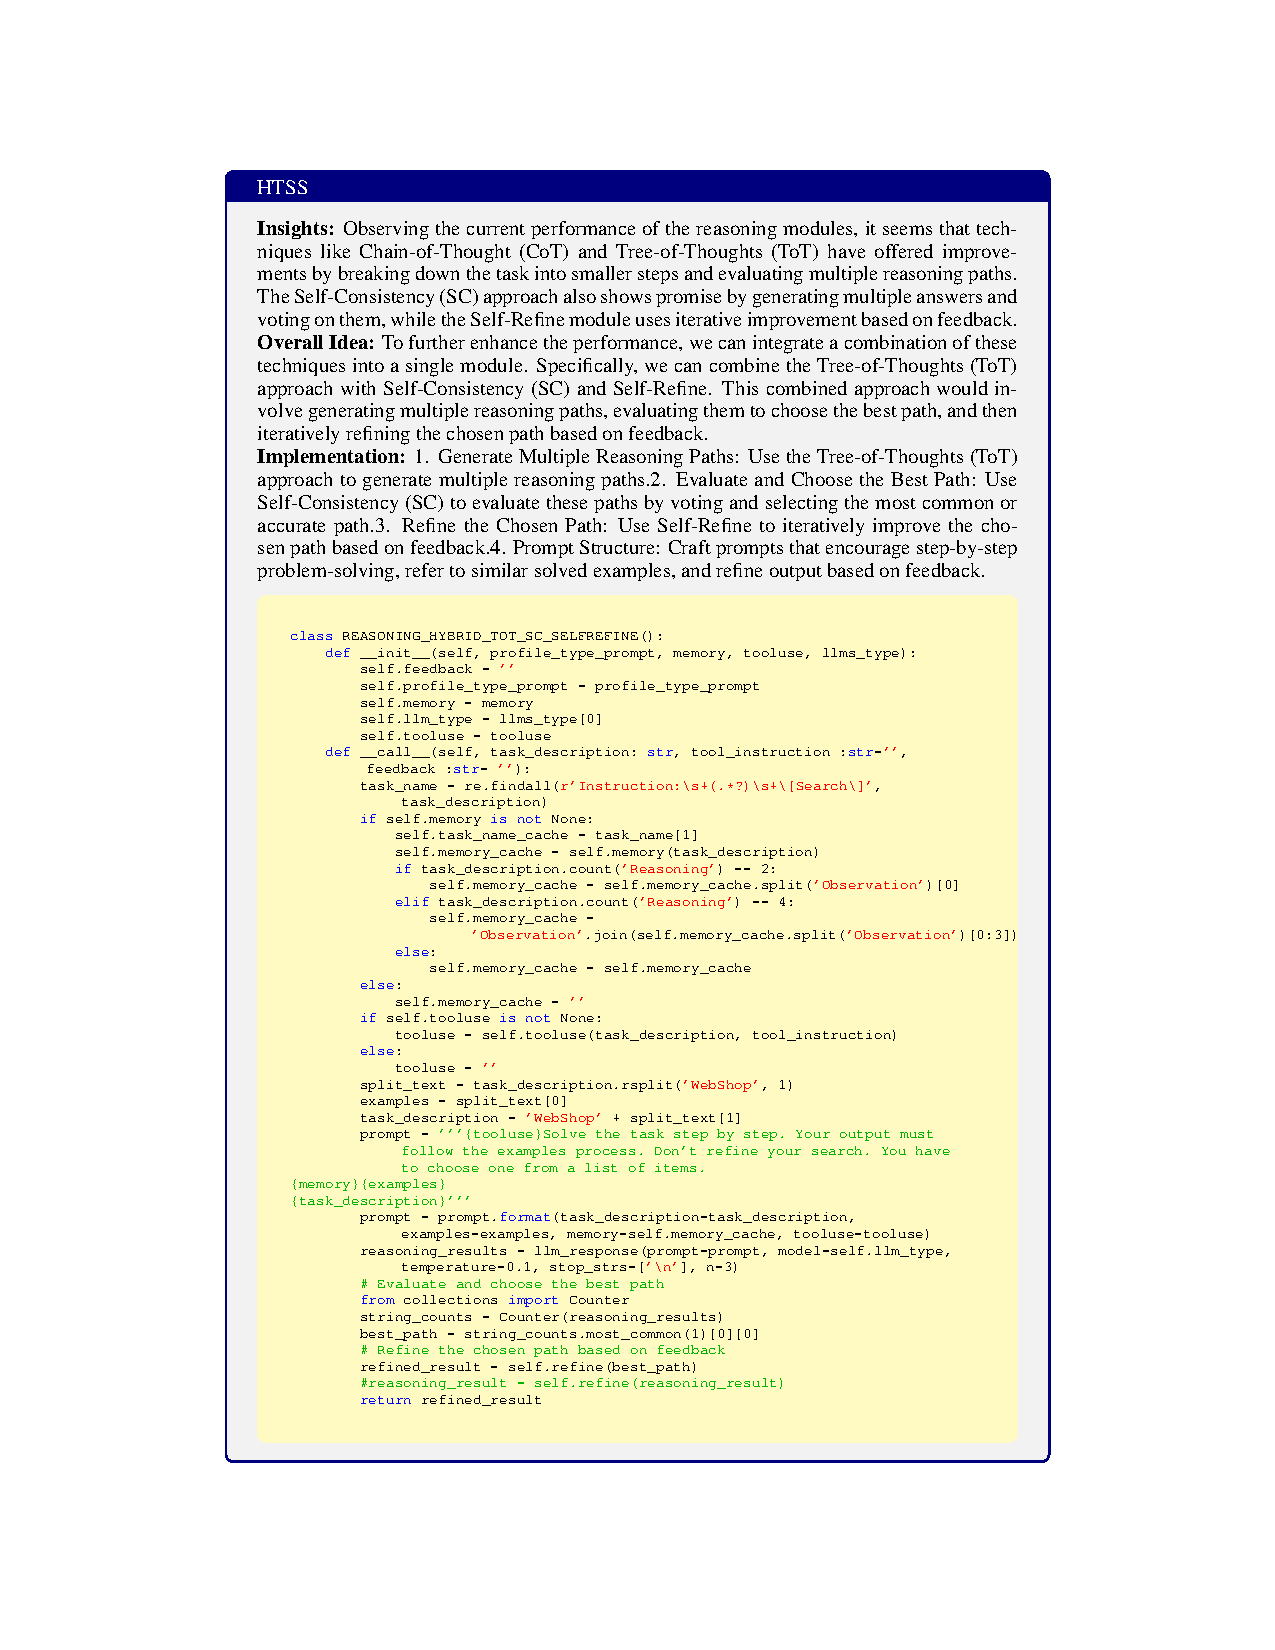
\includegraphics[width=\textwidth]{Figures/new_module_HTSS.pdf}
\caption{New module discovered through AgentSquare search on Webshop.}
\label{New module1}
\end{center}
\end{figure}
\begin{figure}[!t]
\begin{center}
%\fbox{\rule[-.5cm]{0cm}{4cm} \rule[-.5cm]{4cm}{0cm}}
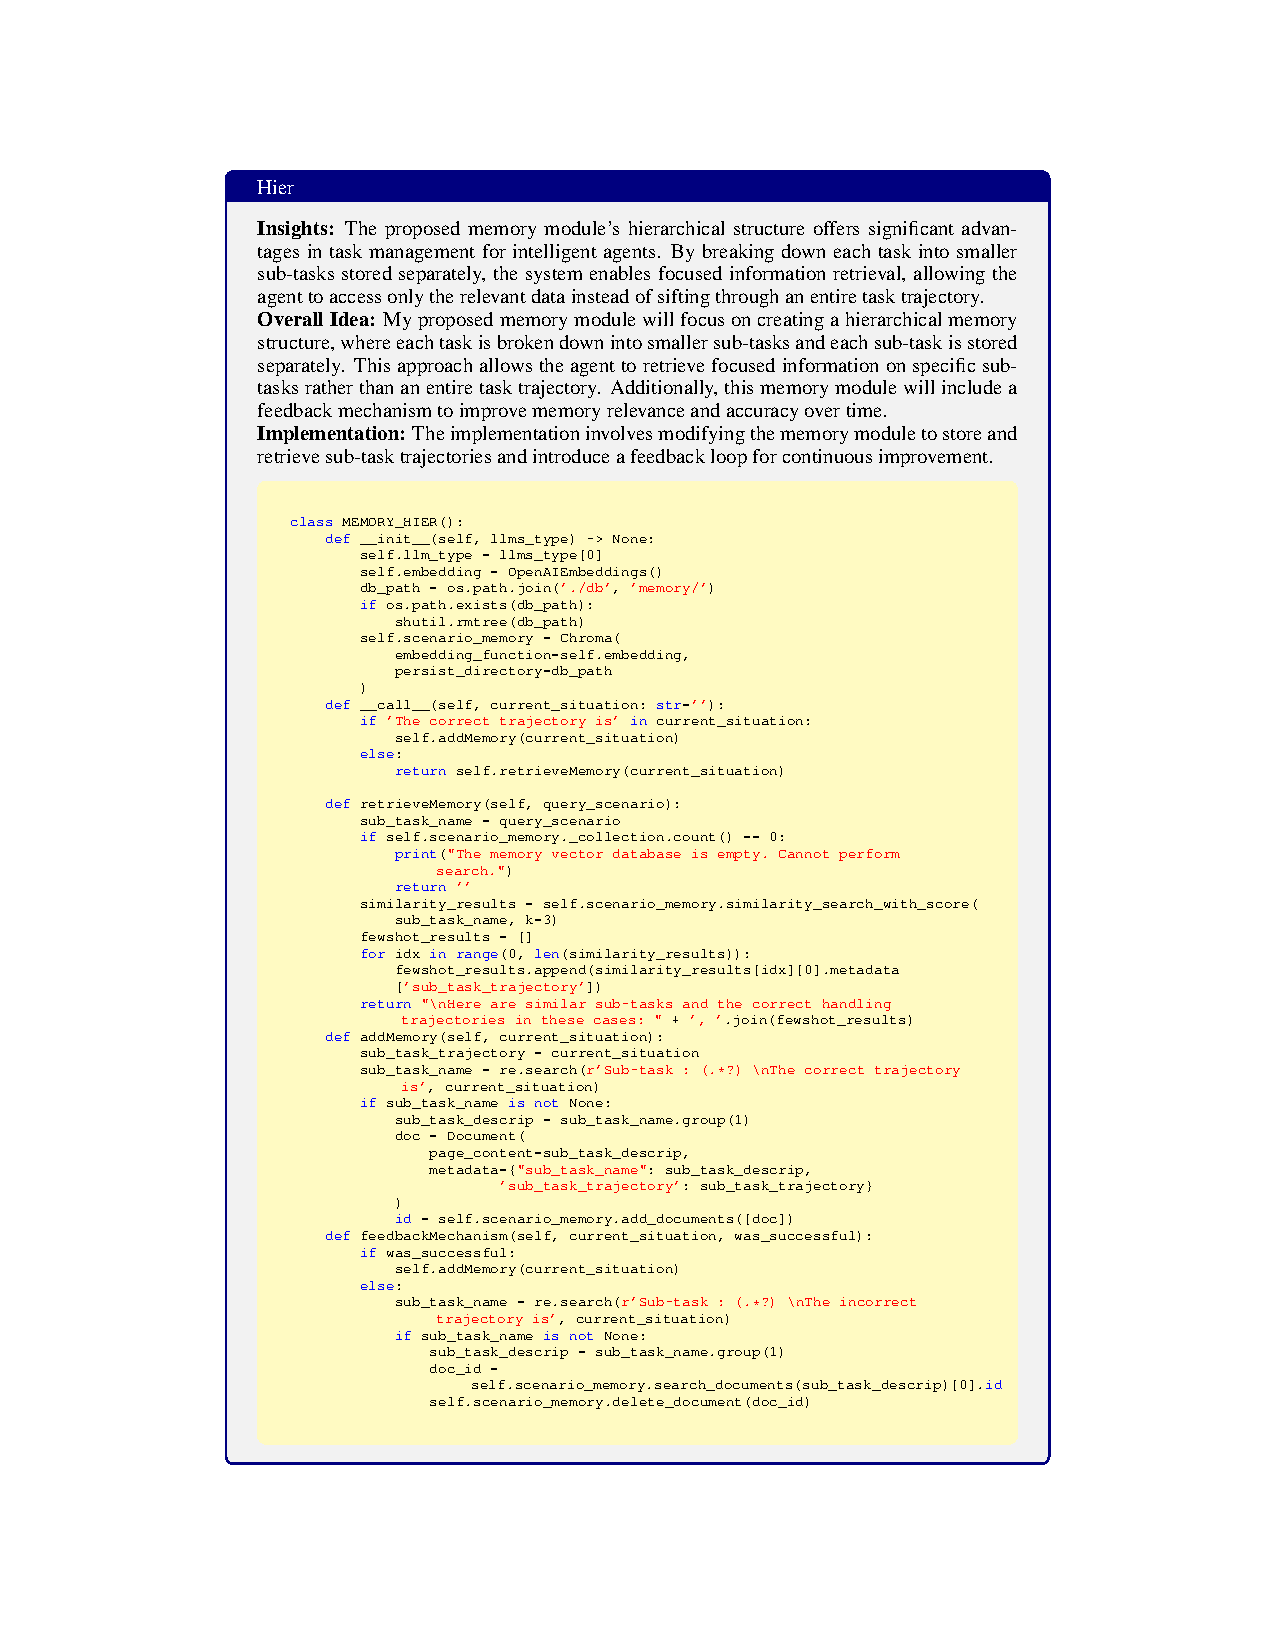
\includegraphics[width=\textwidth]{Figures/new_module_Hier.pdf}
\caption{New module discovered through AgentSquare search on Sciworld.}
\label{New module2}
\end{center}
\end{figure}

\begin{figure}[!t]
\begin{center}
%\fbox{\rule[-.5cm]{0cm}{4cm} \rule[-.5cm]{4cm}{0cm}}
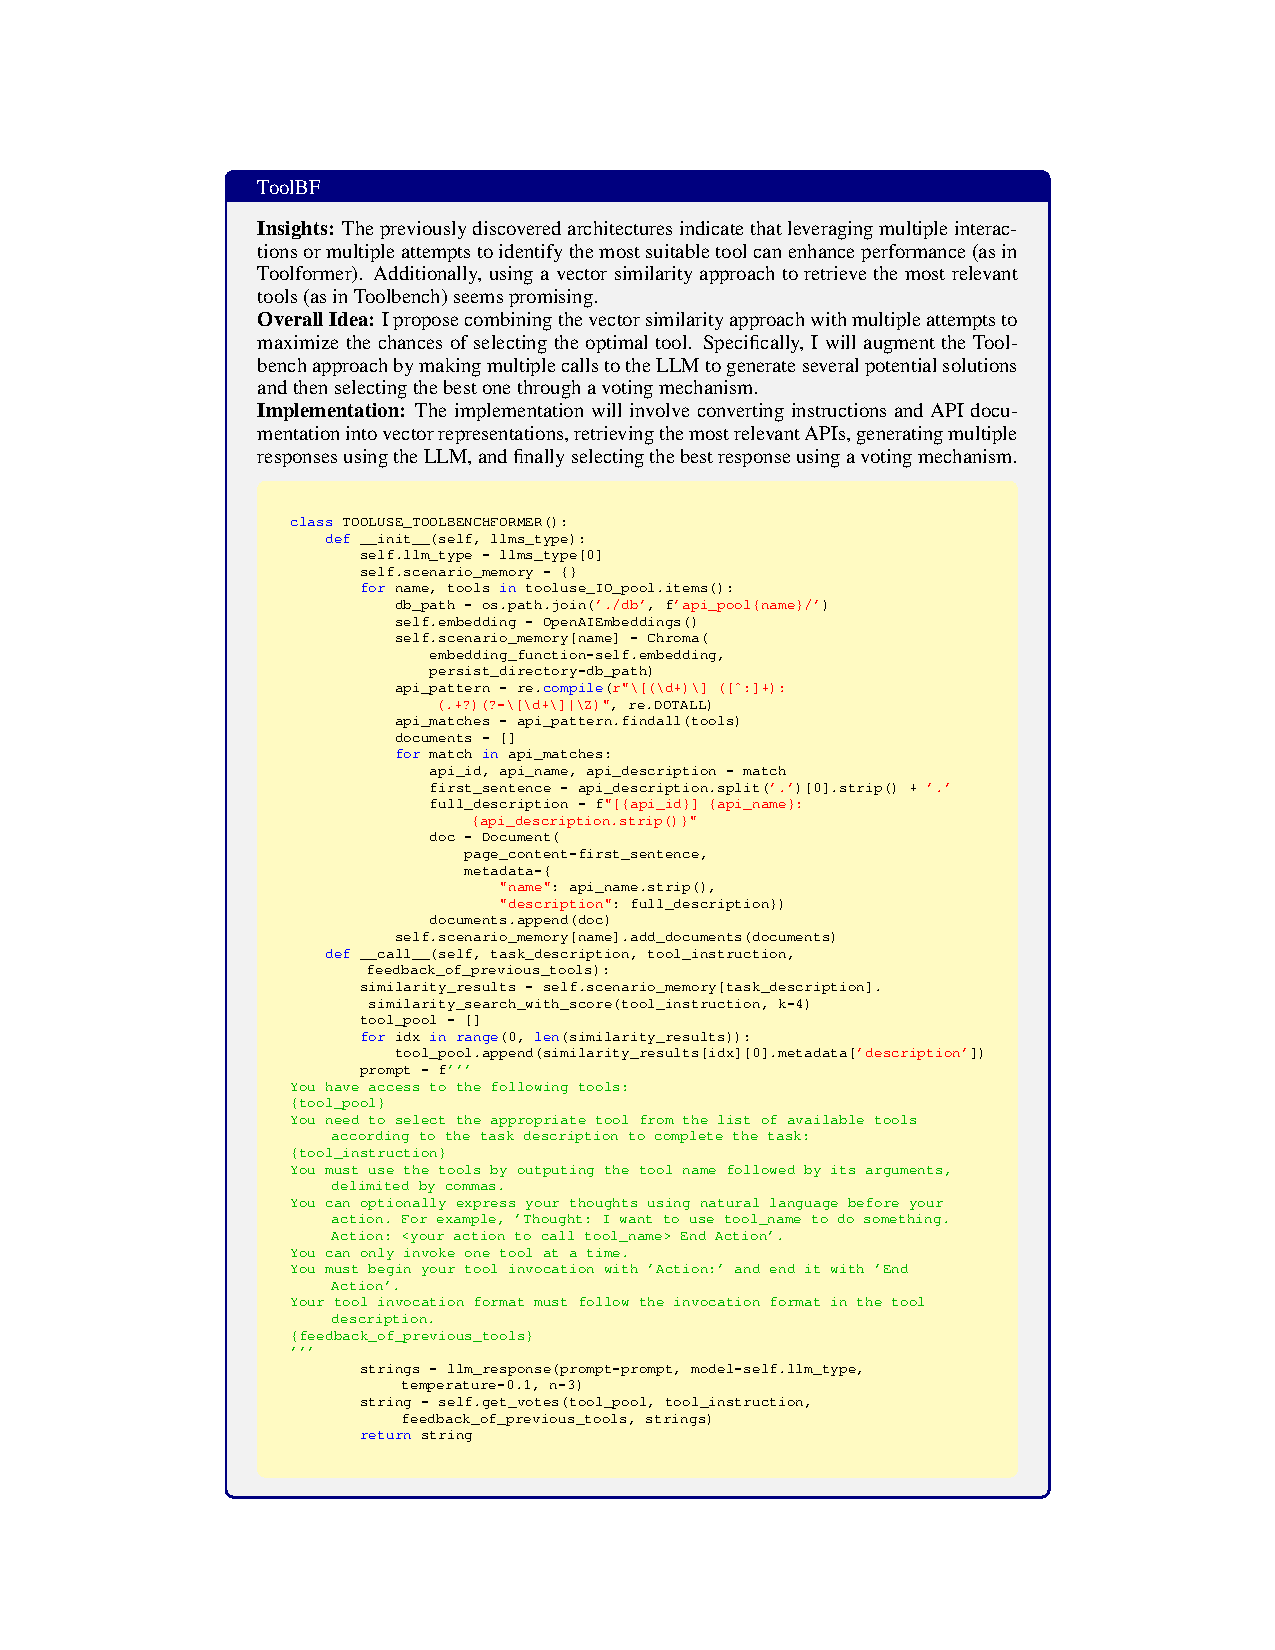
\includegraphics[width=0.98\textwidth]{Figures/new_module_ToolBF.pdf}
\caption{New module discovered through AgentSquare search on M3tool.}
\label{New module3}
\end{center}
\end{figure}
\begin{figure}[!t]
\begin{center}
%\fbox{\rule[-.5cm]{0cm}{4cm} \rule[-.5cm]{4cm}{0cm}}
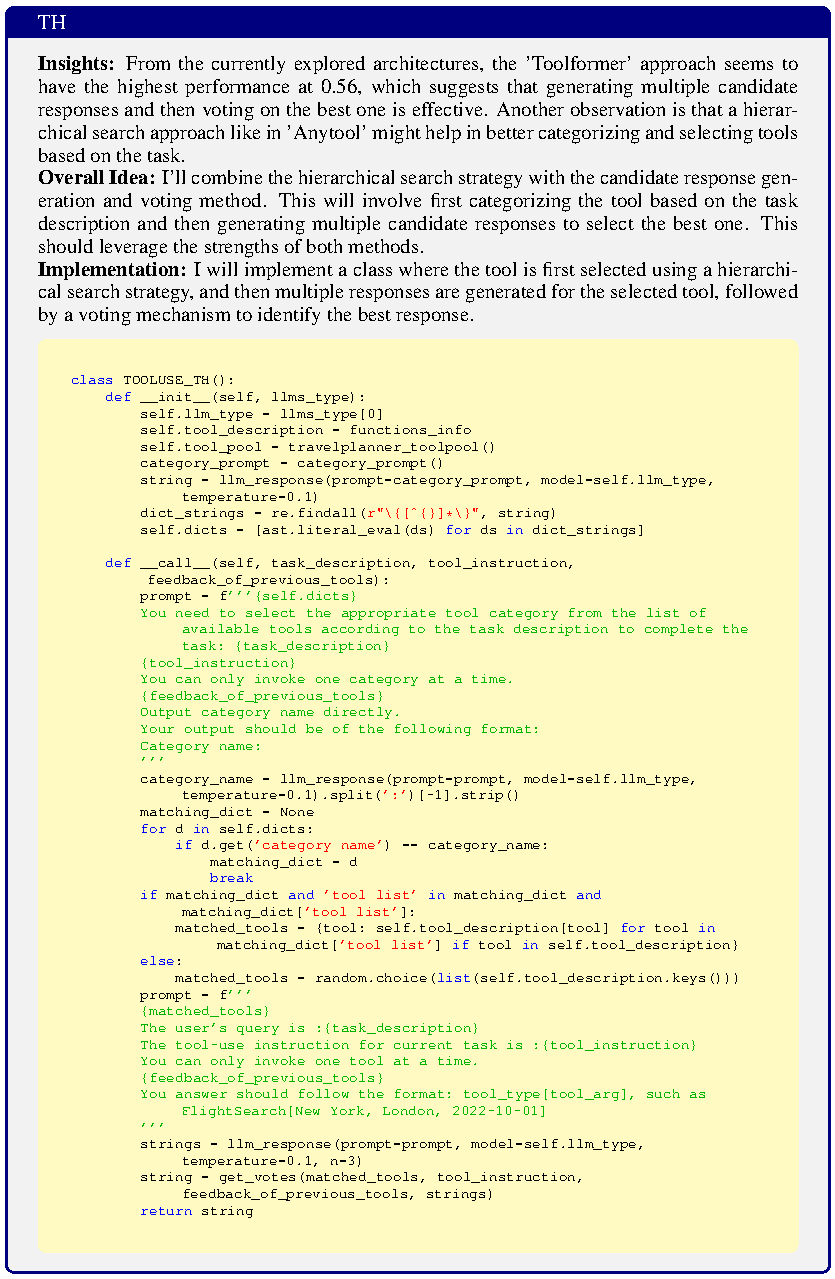
\includegraphics[width=0.98\textwidth]{Figures/new_module_TH.pdf}
\caption{New module discovered through AgentSquare search on Travelplanner.}
\label{New module4}
\end{center}
\end{figure}
\begin{figure}[!t]
\begin{center}
%\fbox{\rule[-.5cm]{0cm}{4cm} \rule[-.5cm]{4cm}{0cm}}
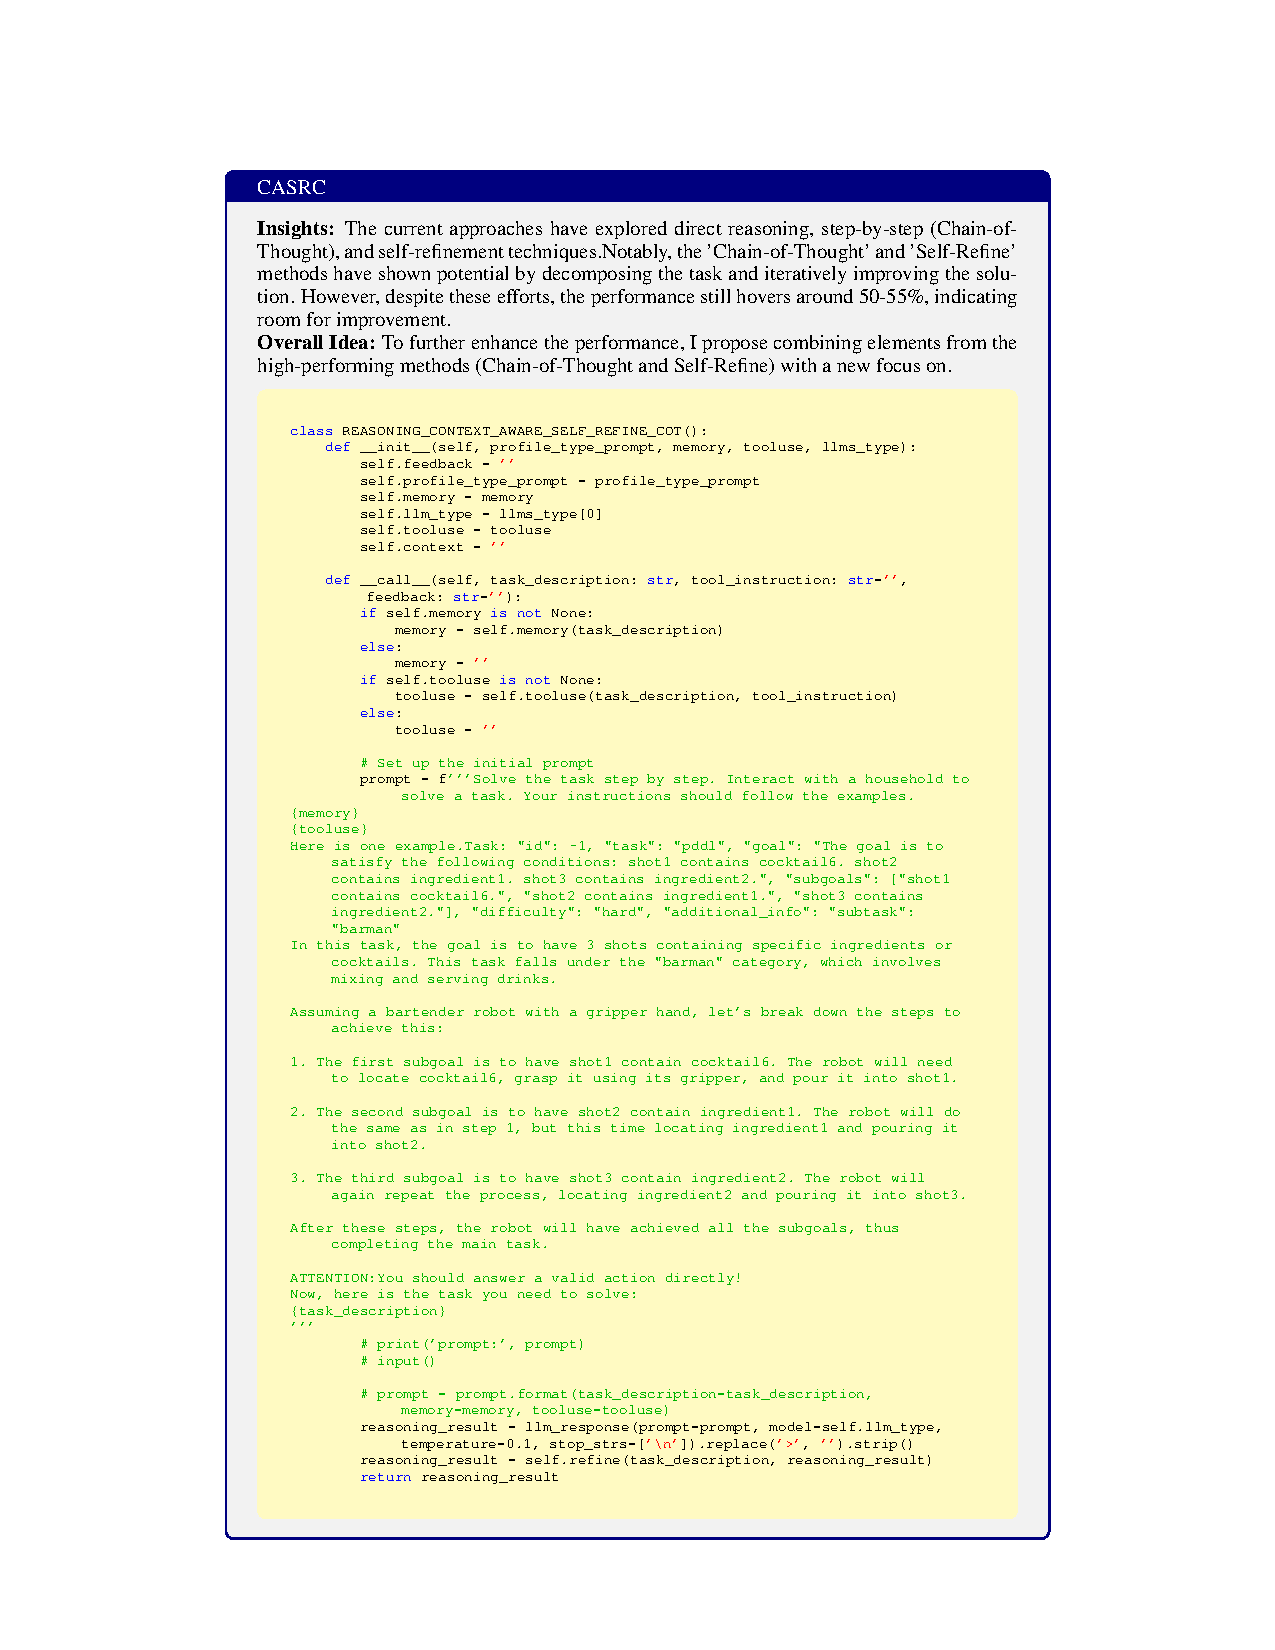
\includegraphics[width=0.95\textwidth]{Figures/new_module_CASRC.pdf}
\caption{New module discovered through AgentSquare search on Pddl.}
\label{New module5}
\end{center}
\end{figure}

\begin{figure}[!t]
\begin{center}
%\fbox{\rule[-.5cm]{0cm}{4cm} \rule[-.5cm]{4cm}{0cm}}
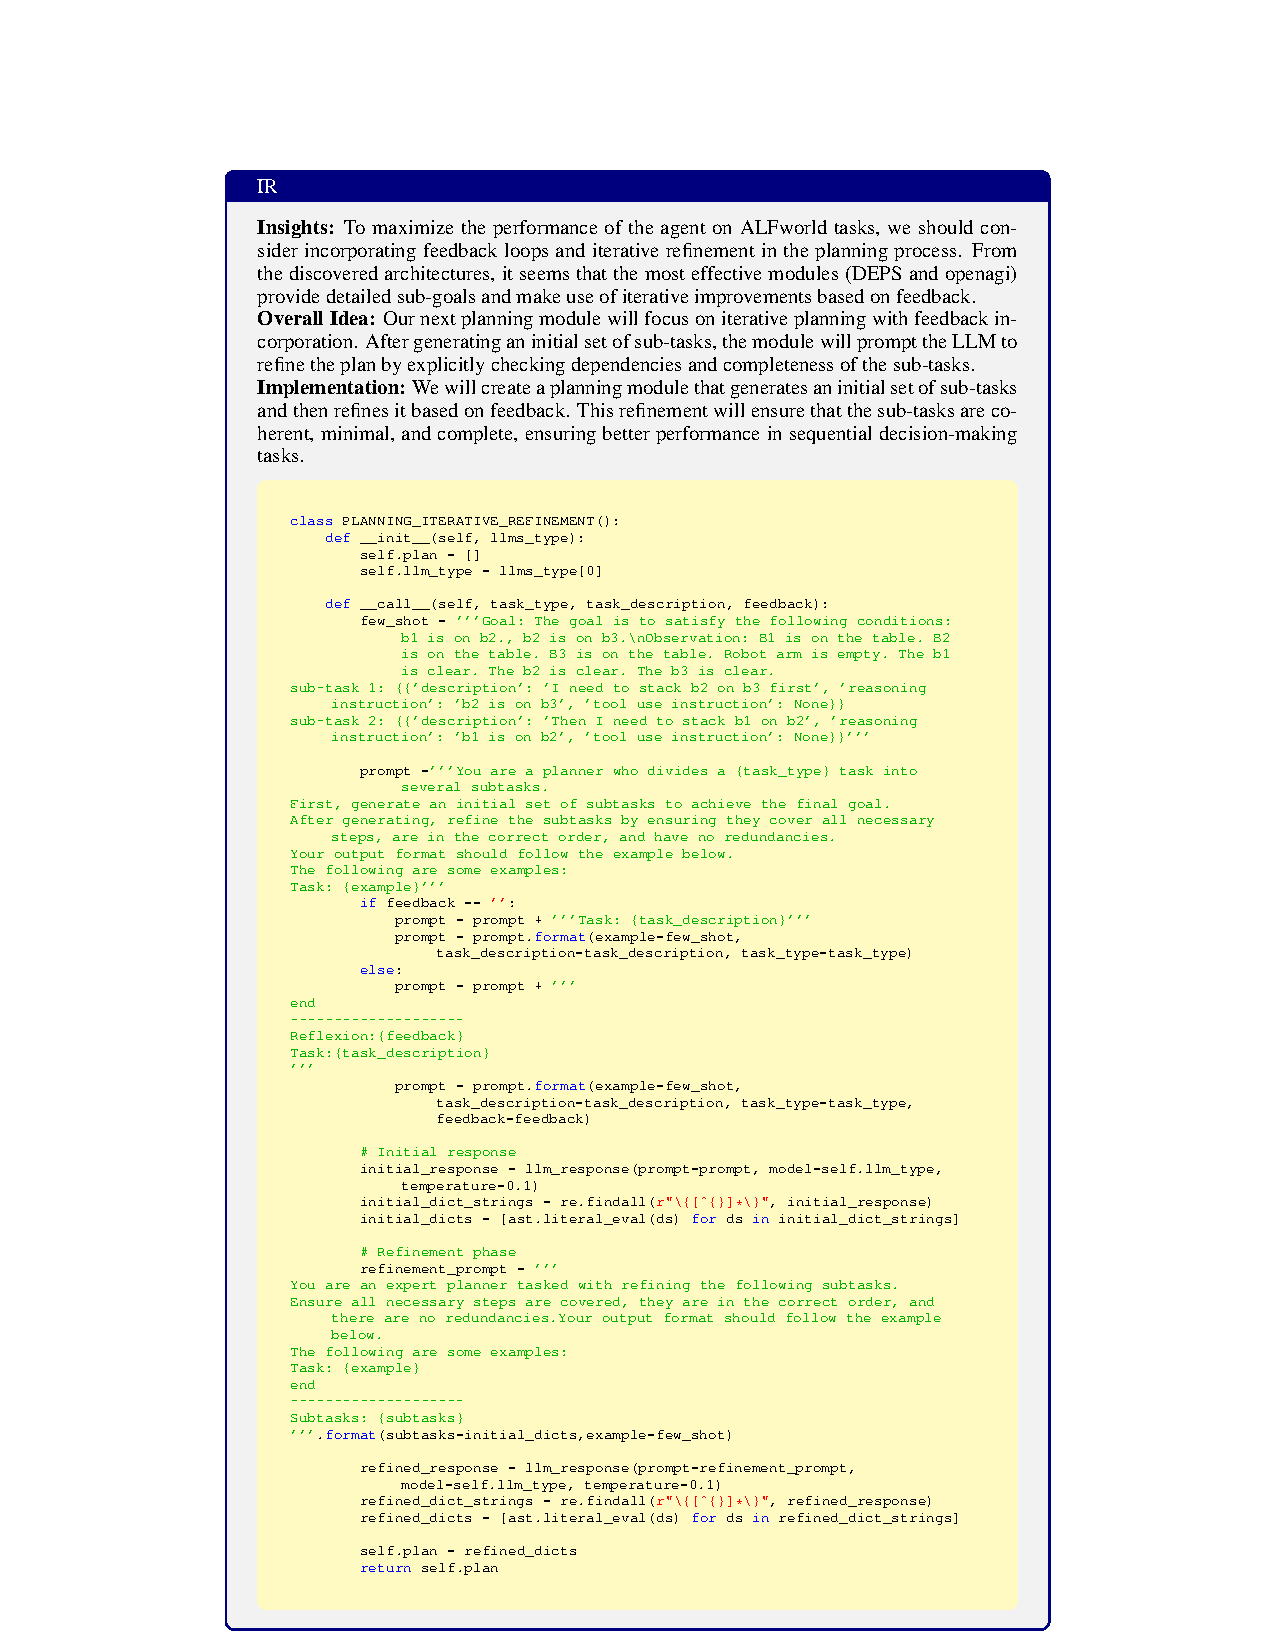
\includegraphics[width=0.89\textwidth]{Figures/new_module_IR.pdf}
\caption{New module discovered through AgentSquare search on Pddl.}
\label{New module6}
\end{center}
\end{figure}

